\documentclass[english,course]{lecture}

\usepackage{listings}
\definecolor{mygreen}{rgb}{0,0.6,0}
\definecolor{mygray}{rgb}{0.5,0.5,0.5}
\definecolor{mymauve}{rgb}{0.58,0,0.82}

\lstset{ %
  backgroundcolor=\color{white},
  basicstyle=\footnotesize,
  breakatwhitespace=false,
  breaklines=true,
  captionpos=b,
  commentstyle=\color{mygreen},
  escapeinside={\%*}{*)},
  extendedchars=true,
  frame=single,
  keepspaces=true,
  keywordstyle=\color{blue},
  language=C,
  %numbers=left,
  numbersep=5pt,
  numberstyle=\tiny\color{mygray},
  rulecolor=\color{black},
  showspaces=false,
  showstringspaces=false,
  showtabs=false,
  stepnumber=2,
  stringstyle=\color{mymauve},
  tabsize=2,
  title=\lstname
}
\usepackage{cleveref}
\usepackage{longtable}
\usepackage{tikz}
\usepackage{amsmath}
\usepackage{adjustbox}
%--------------------------------------------------------------------------
% First, provide some data about this document
\title{lecture notes}
\subtitle{Cybersecurity Specialist}
%\shorttitle{Shortened title} % For headers; if undefined, the usual title will be used
\ccode{CS0424IT} % Most of these data are not compulsory
% \subject{Subject of the Talk}
\author{Simone La Porta}
% \spemail{speaker@email.com}
% \email{email@email.com}
% \speaker{Speaker's name}
\date{27}{05}{2024}
\dateend{13}{09}{2024}
% \conference{Lecture hall 7}
% \place{University of Physics}
\flag{\href{https://github.com/simone0509/CS0424IT}{
\includegraphics[scale=0.06]{images/github_logo.png}} \\ Written in \LaTeX}
% \attn{Place anything here to gather your readers' attention. This could be a warning, a disclaimer, a license, or, more likely, some helpful suggestions for your readers.}
% \morelink{https://github.com/simone0509/CS0424IT}
%-----------------------------------------------------------------------------


% And then begin your document
\begin{document}

\part{Unit 1: Fundamentals of Ethical Hacking}
\section{Introduction and Virtual Machines}\lecture[4 hours]{27}{05}{2024}

The Cybersecurity Specialist course aims to train professionals in the field of information security. These individuals will possess strong technical skills, providing added value to companies in the fight against cybercrime. The course is divided into three units:
\begin{enumerate}
    \item \textbf{Unit 1} focuses on the theoretical prerequisites and technical skills necessary for an Ethical Hacker. It covers topics such as networking, operating systems, and an introduction to programming;
    \item \textbf{Unit 2} centers on the phases of Penetration Testing, exploring the tools and techniques used by hackers in the real world;
    \item \textbf{Unit 3} provides students with a comprehensive understanding of how to monitor security events, manage ongoing attacks, and adopt best practices at the enterprise level to minimize the impact on business activities.
\end{enumerate}

In the past century, computing and the web were primarily the domain of experts, including hackers. The term \emph{hacker}, often associated with digital piracy, encompasses three distinct types of hackers:
\begin{itemize}
    \item \textbf{White Hat Hackers}, also known as "Ethical Hackers," operate with a strict adherence to ethical standards. Their work involves improving security with the consent of the system owner;
    \item \textbf{Grey Hat Hackers} operate in a legal and ethical gray area. They often act without the owner's permission but with the intent of improving security. While their actions can uncover vulnerabilities, they can also be controversial and sometimes illegal;
    \item \textbf{Black Hat Hackers} are criminals who break into computer networks with malicious intent. They may deploy malware to destroy files, steal information, hold computers hostage, or pilfer passwords, credit card numbers, and other personal data. Their motivations are typically opportunistic, such as financial gain. Stolen data is often sold on the dark web, where items like credit card details, online payment system access, medical records, and even streaming service accounts are traded.
\end{itemize}

An Ethical Hacker is a cybersecurity expert capable of simulating cyber-attacks to identify potential vulnerabilities in a company's systems. These simulations, known as \emph{Penetration Tests}, are crucial for detecting and fixing security issues in digital networks, software, and devices, thereby protecting enterprises and public entities from cybercriminal activities. Key responsibilities of an Ethical Hacker include:
\begin{itemize}
    \item Conducting penetration tests on IT infrastructures and web applications;
    \item Ensuring the security of sensitive and private data, such as payment details, login credentials, and passwords.
\end{itemize}

It is crucial to emphasize that penetration testing should only be performed with the formal consent of the system or network owner. Conducting such tests without permission is illegal and can lead to severe legal consequences.


\subsection{Virtualization Process}
Virtual machines (VMs) are emulations of computer systems that provide the functionality of a physical computer. They run on a physical host machine and are managed by a virtualization layer. The process of creating and managing VMs is known as virtualization (\Cref{fig:virtualization}).
Virtualization involves several key steps:

\begin{enumerate}
    \item \textbf{Hypervisor Installation:} The hypervisor, also known as the Virtual Machine Monitor (VMM), is installed on the host machine. The hypervisor can be of two types:
    \begin{itemize}
        \item \textbf{Type 1 (Bare Metal):} Runs directly on the host's hardware.
        \item \textbf{Type 2 (Hosted):} Runs on top of an existing operating system.
    \end{itemize}
    \item \textbf{Resource Allocation:} The hypervisor allocates resources (CPU, memory, storage, and network) from the physical host to each VM.
    \item \textbf{VM Creation:} Virtual machines are created by defining their virtual hardware specifications (number of CPUs, amount of memory, disk size, etc.).
    \item \textbf{Operating System Installation:} An operating system is installed on the virtual machine, just as it would be on a physical machine.
    \item \textbf{VM Management:} The hypervisor manages the execution of VMs, handles resource allocation dynamically, and ensures isolation between VMs.
\end{enumerate}

\begin{figure}
    \begin{center}
        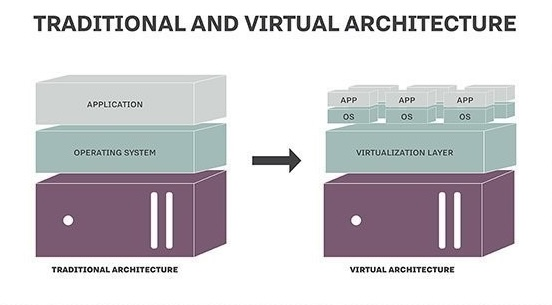
\includegraphics[width=\textwidth]{images/virtualization.jpg}
        \caption{Traditional vs Virtual architecture.}
        \label{fig:virtualization}
    \end{center}
\end{figure}


\subsubsection{Virtual Hardware}
A virtual machine emulates physical hardware components such as:
\begin{itemize}
    \item \textbf{CPU:} Virtual CPUs (vCPUs) are assigned to the VM by the hypervisor.
    \item \textbf{Memory:} Virtual memory is allocated from the host's physical memory.
    \item \textbf{Storage:} Virtual disks are created using files on the host's storage system.
    \item \textbf{Network:} Virtual network interfaces connect VMs to the host's network and to other VMs.
\end{itemize}

\subsubsection{Hypervisor Role}
The hypervisor plays a critical role in:
\begin{itemize}
    \item \textbf{Resource Management:} Dynamically allocating resources to VMs based on their needs.
    \item \textbf{Isolation:} Ensuring that each VM operates independently and securely.
    \item \textbf{Efficiency:} Optimizing resource usage to maximize the performance of VMs.
\end{itemize}

\subsubsection{Execution Flow}
The execution flow of a VM includes:
\begin{enumerate}
    \item \textbf{Boot Process:} The VM goes through a boot process similar to a physical machine, loading its operating system from the virtual disk.
    \item \textbf{Application Execution:} Applications run within the VM, utilizing the virtualized hardware.
    \item \textbf{Hypervisor Interaction:} The VM interacts with the hypervisor for tasks like I/O operations, which the hypervisor translates to the physical hardware.
\end{enumerate}

\subsubsection{Benefits of Virtualization}
Virtualization offers several advantages:
\begin{itemize}
    \item \textbf{Cost Efficiency:} Reduces the need for physical hardware.
    \item \textbf{Scalability:} Easily create, modify, and delete VMs as needed.
    \item \textbf{Isolation:} Provides a secure and isolated environment for each VM.
    \item \textbf{Resource Utilization:} Maximizes the usage of physical resources.
\end{itemize}

Virtualization is a powerful technology that enables the efficient use of hardware resources, providing flexibility, scalability, and isolation. Virtual machines are an integral part of modern computing environments, supporting a wide range of applications from development to production systems.

\section{Networking}\lecture[4 hours]{28}{05}{2024}\lecture[4 hours]{29}{05}{2024}
\subsection{Network Categories: Geographical and Topological}
\subsubsection{Geographical Networks}

Networks can be categorized based on the geographical distance between devices. The primary types of geographical networks include:

\paragraph{WAN - Wide Area Network}
Wide Area Networks (WANs) connect computers over large distances, covering extensive geographical areas. WANs use various transmission methods such as satellites, fiber optics, and cables. The quintessential example of a WAN is the Internet, which allows computers in different continents to communicate within seconds.

\paragraph{LAN - Local Area Network}
Local Area Networks (LANs) connect computers within a smaller geographical area, such as the floors of a building in a company. LANs are popular due to their high speed and relative ease of installation.

\paragraph{PAN - Personal Area Network}
Personal Area Networks (PANs) cover very limited areas, such as the connection between a mobile phone and a computer.

\subsubsection{Topological Networks}

Networks can also be categorized based on their physical configuration. The primary types of topological networks include the following, also shown in \Cref{fig:net_topo}.

\begin{figure}[h]
    \centering
    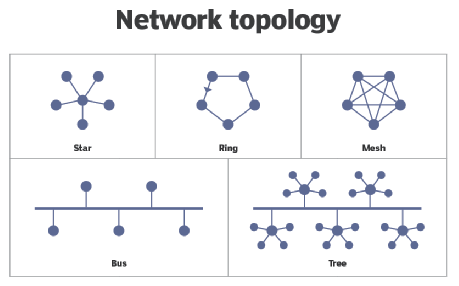
\includegraphics[width=\textwidth]{images/network_topology.png}
    \caption{Network topologies.}
    \label{fig:net_topo}
\end{figure}

\paragraph{Bus Topology}
In a bus topology, devices share a single transmission channel, typically a single cable. One of the advantages of bus topology is its simplicity and ease of implementation.

\paragraph{Ring Topology}
In a ring topology, devices are connected in a circular manner. These networks are more complex and expensive than bus networks and are generally used in enterprise environments for corporate LANs.

\paragraph{Star Topology}
In a star topology, devices are individually connected to a central device, such as a switch or router, using dedicated cables or other physical media. Each computer has a dedicated link to the central device and can communicate with other devices through it. Star networks are the most widely used due to their performance and security characteristics.

Understanding the different types of networks, both geographical and topological, is essential for designing and implementing efficient and secure network infrastructures. WANs, LANs, and PANs cater to different geographical scopes, while bus, ring, and star topologies offer various configurations to meet specific organizational needs.


\subsection{Basic Networking Concepts}

A computer network enables and facilitates communication between people, applications, and servers regardless of their geographical location. The Internet is the largest example of a computer network that we use on a daily basis. In a computer network, machines communicate with each other using communication \textit{protocols}, which ensure communication between computers with different hardware and software.

\subsubsection{Data Transmission}

Communication occurs through an exchange of data, or information, which is transported in the form of \textit{packets}. Packets are streams of bits exchanged via electrical signals over a physical medium. The physical medium can be a LAN (local area network) cable or, very commonly, the air in a Wi-Fi network.

\begin{figure}[h]
    \centering
    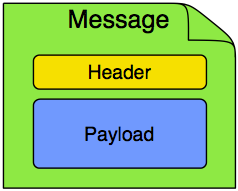
\includegraphics[width=0.4\textwidth]{images/message.png}
    \caption{Structure of a Packet: Header and Payload.}
    \label{fig:packet_structure}
\end{figure}

\subsubsection{Packet Structure}

A \textit{packet} has a defined structure as shown in \Cref{fig:packet_structure}. The \textit{Header} depends on the protocol used in the communication. Its task is to ensure that the receiving computer can interpret the \textit{Payload} and manage the communication. The \textit{Payload}, on the other hand, is the actual information. For instance, it could be a message, or part of a message sent from one computer to another, an email, or other data.

\subsection{The ISO/OSI Model}

To standardize network communication, in 1984 the International Organization for Standardization (ISO) published a theoretical model subsequently called the \textit{Open System Interconnection (OSI)} model. The ISO/OSI model is used as a theoretical reference. It is based on a stack of 7 layers, also called \textit{layers}, where each layer serves the upper layer and has exclusive protocols.

\begin{figure}[h]
    \centering
    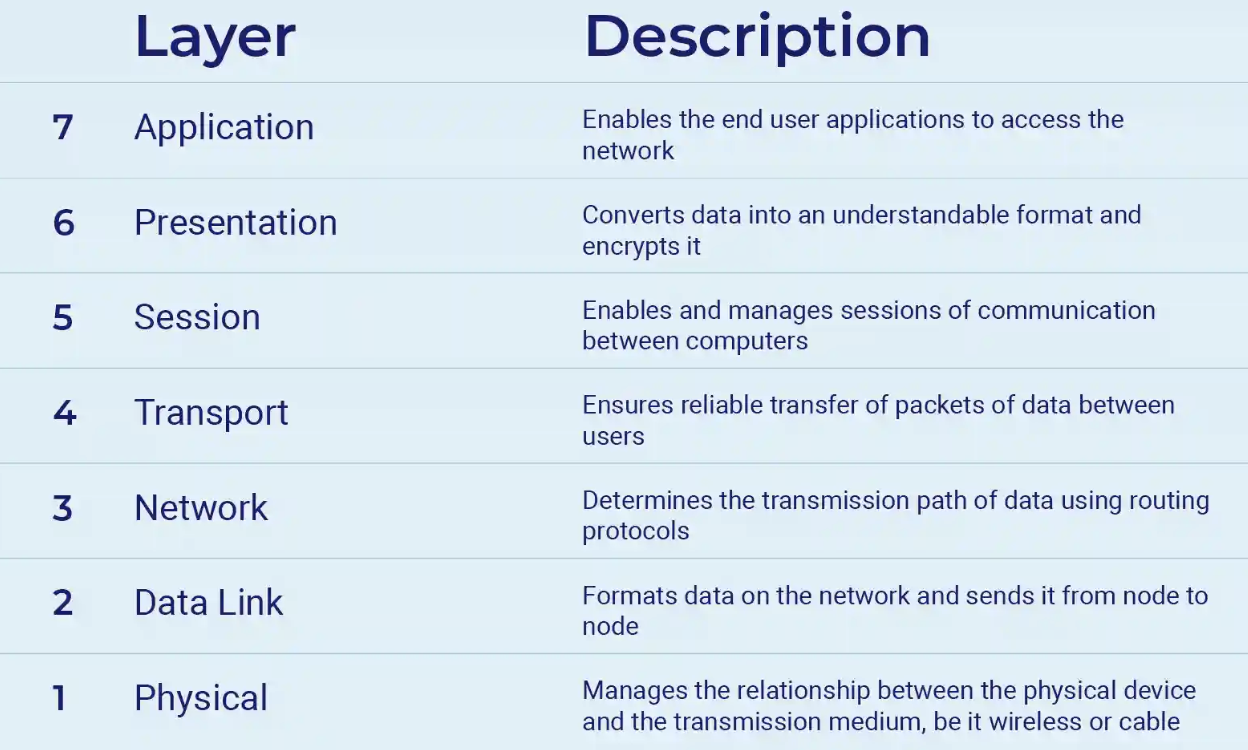
\includegraphics[width=\textwidth]{images/layers_osi.png}
    \caption{The ISO/OSI Model Layers.}
    \label{fig:osi_layers}
\end{figure}

In a communication between two computers, the data follows the logical model as represented by the line in \Cref{fig:osi_model}.

\begin{figure}[h!]
    \centering
    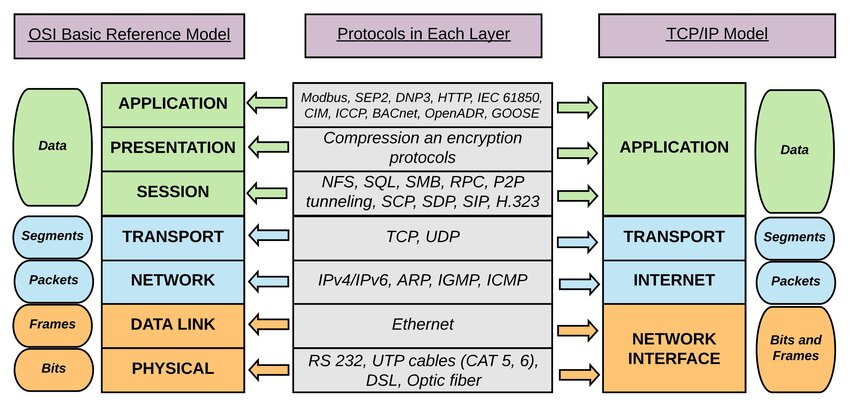
\includegraphics[width=\textwidth]{images/iso_osi_tcp.png}
    \caption{The ISO/OSI vs TCP/IP model.}
    \label{fig:osi_model}
\end{figure}

Note that the ISO/OSI model is a theoretical model to be used as a reference. In practice, applications use the \textit{TCP/IP} model, which slightly varies from the theoretical ISO/OSI model.

The differences between TCP/IP and the ISO/OSI model are depicted in \Cref{fig:osi_model} and summarized in \Cref{fig:tcp_vs_osi}. For theoretical study of concepts, we will follow the notions of the ISO/OSI model.

\begin{figure}[h!]
    \centering
    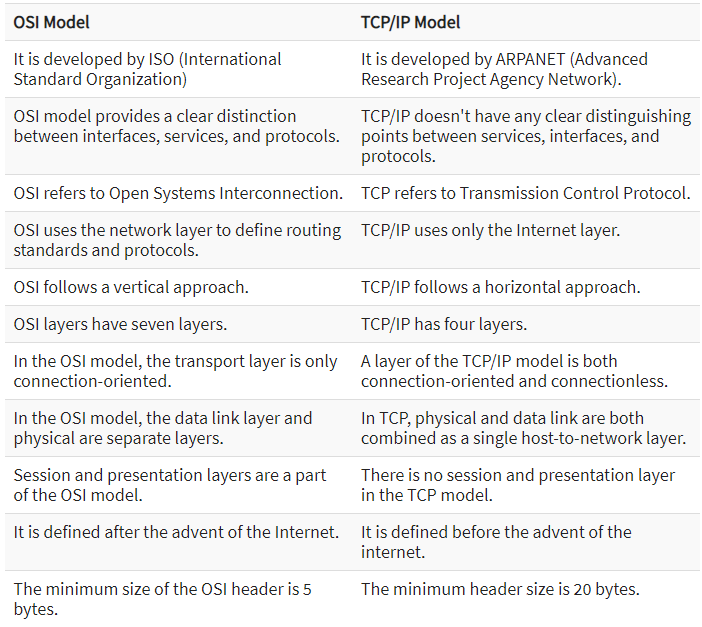
\includegraphics[width=\textwidth]{images/tcp_vs_osi.png}
    \caption{The ISO/OSI vs TCP/IP model.}
    \label{fig:tcp_vs_osi}
\end{figure}


\subsubsection{\textbf{Physical Layer}}
The physical layer is responsible for the transmission of raw data bits over a physical medium. This transmission can occur via various types of cabling, such as copper wires or fiber optics. Data from higher layers of the source computer is segmented and sent to the physical layer of the receiving computer in the form of bits.

\paragraph{Bits and Binary System}
The bit, short for binary digit, is the basic unit of information in computing, represented as either '0' or '1'. Unlike the decimal system, which uses ten digits (0-9), computers operate using the binary system. Consequently, information is transmitted over a physical cable as a sequence of binary digits, for example, 10010010 10011110, etc.

\subsubsection{\textbf{Data Link Layer}}
The Data Link Layer utilizes the services of the physical layer to send and receive bits over communication channels. Packets at this layer are referred to as frames. The main functions of the Data Link Layer include:

\begin{itemize}
    \item Providing an interface to the Network Layer (Layer 3)
    \item Handling transmission errors
    \item Regulating the flow of bits between two communicating devices
\end{itemize}

The Data Link Layer plays a crucial role by defining protocol standards such as IEEE 802.3 for Ethernet (wired connections) and IEEE 802.11 for Wireless connections.

\paragraph{MAC Address}
In a computer network, two personal computers communicate at the Data Link Layer using what is called a physical address or more commonly, a MAC Address. The MAC address is a 48-bit identifier typically represented in hexadecimal format. Below is a table showing the conversion between binary and hexadecimal systems:

\begin{table}[h]
    \centering
    \begin{tabular}{|c|c|}
        \hline
        \textbf{Binary} & \textbf{Hexadecimal} \\
        \hline
        0000 & 0 \\
        0001 & 1 \\
        0010 & 2 \\
        0011 & 3 \\
        0100 & 4 \\
        0101 & 5 \\
        0110 & 6 \\
        0111 & 7 \\
        1000 & 8 \\
        1001 & 9 \\
        1010 & A \\
        1011 & B \\
        1100 & C \\
        1101 & D \\
        1110 & E \\
        1111 & F \\
        \hline
    \end{tabular}
    \caption{Binary to Hexadecimal Conversion}
    \label{tab:bin_hex}
\end{table}

An example of a MAC Address is 00:AA:11:BB:22:CC. The MAC address is a unique identifier assigned to the network interfaces of devices.

\paragraph{Ethernet Frame Structure}
The structure of an Ethernet 802.3 frame includes fields for the Destination MAC Address and the Source MAC Address. These fields are automatically populated with the MAC addresses of the source and destination when an exchange of information begins at the Data Link Layer.

\paragraph{Role of Switches}
Switches are vital network devices for communication but come with certain disadvantages. They route broadcast packets across the entire network. Broadcast packets are sent to a specific MAC address, FF:FF:FF:FF:FF:FF, which is received by the switch and routed to all nodes connected to it. This creates what is known as a broadcast domain.

A broadcast domain includes all the devices on a network segment that receive broadcast frames from any device within the segment. In a large network with numerous devices, this can cause significant latency issues.

\paragraph{Address Resolution Protocol (ARP)}
ARP, or Address Resolution Protocol, is a network protocol used to map IP addresses to MAC addresses within a local network. Its primary functions include:

\begin{itemize}
    \item \textbf{ARP Request}: A device broadcasts an ARP request on the local network, asking for the MAC address associated with a specific IP address.
    \item \textbf{ARP Reply}: The destination device responds with a packet containing its MAC address associated with the requested IP address.
    \item \textbf{ARP Cache}: Devices maintain an ARP table or ARP cache that stores IP-to-MAC address mappings.
\end{itemize}


ARP is crucial for communication within the same local network. When a device needs to send data to another device within the same subnet, it uses ARP to discover the MAC address corresponding to the destination IP address.

\paragraph{Virtual LAN (VLAN)}\lecture[4 hours]{30}{05}{2024}
Switches allow the segmentation of broadcast domains through the creation of Virtual LANs (VLANs). A VLAN is a logical grouping of hosts and network devices. VLANs are created by adding a "tag" or VLAN ID to the switch ports, or by mapping the MAC address of the host to the VLAN ID.

Assume we want to restrict communication and the broadcast domain to hosts A, B, and C. We create a VLAN identified by ID 100 and associate the MAC addresses of hosts A, B, and C with that VLAN.

When host A sends a packet to the broadcast address, it will only be received by hosts B and C. Therefore, VLANs segment broadcast domains and eliminate latency issues in large networks.


VLANs are essential for managing broadcast domains within a network. By associating specific MAC addresses with VLAN IDs, we can ensure that broadcast traffic is limited to only those hosts within the same VLAN, thus improving network efficiency and reducing latency.


\subsubsection{\textbf{Network Layer}}
In networking, just as there are specific devices at the Data Link Layer that facilitate communication between personal computers on the same network, there are devices at the Network Layer, such as router-gateways, that enable data routing between personal computers connected to different networks. For instance, consider the following network configuration:

\paragraph{Role of the Router}
A switch operates at Layer 2 and does not route packets to other networks because it forwards packets based on MAC addresses rather than IP addresses. The solution is to use a Layer 3 device like a router-gateway.

The router receives the packet from the switch and checks its routing table to determine which of its interfaces to forward the packet to reach the destination network.

\paragraph{Example of Router Operation}
To better understand how a router-gateway functions, consider a router connected with three interfaces to three different networks:

If a personal computer on network $2.228.1.0$ wants to send a packet to a PC on network $2.175.1.0$, the packet will be sent to the router, which will check its routing table to see which interface to use to forward the packet.

In a network, computers interact using both MAC and IP addresses. For example, if PC A wants to send a packet to PC B, it will structure the packet as follows:

\begin{itemize}
    \item The destination IP address of B in the datagram header (Layer 3).
    \item The MAC address of the router as the destination in the frame header (Layer 2). The router, in this case, is the "next hop."
    \item Its IP address as the source in the datagram header.
    \item Its MAC address as the source in the frame header.
\end{itemize}

The router will receive the packet and set:
\begin{itemize}
    \item The destination MAC address to that of B.
    \item The source MAC address to that of its corresponding interface.
\end{itemize}

Routers play a crucial role in network communication by enabling the routing of data between different subnets. This process involves intricate interactions between Layer 2 (MAC addresses) and Layer 3 (IP addresses) addressing schemes, ensuring seamless communication across diverse network segments.

\subsubsection{\textbf{Transport Layer}}
The transport layer, also known as layer 4 in the OSI model, is responsible for establishing a logical connection or channel between applications on different computers. It ensures the reliable transmission of data packets between a source and a destination. Packets may get lost during transmission due to network congestion, communication errors, or network issues. In some scenarios, minor transmission issues are tolerable, such as in phone conversations or video streaming, where a lost packet might result in a brief glitch. However, for activities like financial transactions or logging into a portal, it's crucial that communication is lossless.

\paragraph{Protocols in the Transport Layer}
The transport layer provides two fundamental protocols for communication between hosts:
\begin{itemize}
    \item \textbf{TCP (Transmission Control Protocol)}: TCP guarantees data traffic control and reliable delivery to the recipient, making it more secure for applications requiring guaranteed packet delivery. The reliability of TCP is due to its connection-oriented nature, which establishes a communication channel before data exchange. TCP follows a three-step process called the \textit{three-way handshake} to establish this connection.
    \begin{enumerate}
        \item The client initiating the connection sends a TCP packet with the SYN flag set and a random sequence number.
        \item The server responds with a packet that has both SYN and ACK flags set, along with its own sequence number and an acknowledgment number equal to the client's sequence number plus one.
        \item The client completes the synchronization by sending a packet with the ACK flag set, acknowledging the server's sequence number.
    \end{enumerate}
    \item \textbf{UDP (User Datagram Protocol)}: UDP is a connectionless protocol that does not require establishing a communication channel before data exchange. It is more lightweight and faster, suitable for activities requiring data streaming (e.g., video or audio). However, it does not guarantee packet delivery.
\end{itemize}


\paragraph{Ports and Services}
To identify the target process or service for a given packet, both TCP and UDP use ports, represented as \texttt{<ip>:<port>}. While the IP identifies the destination machine, the port provides information about the service. Ports can be categorized into:

\begin{itemize}
    \item \textbf{Well-known ports}: Used for standard services, ranging from 0 to 1023.
    \item \textbf{High ports}: Used for non-standard services, ranging from 1024 to 65535.
\end{itemize}

\begin{table}[h]
    \centering
    \begin{tabular}{|c|c|}
        \hline
        \textbf{Protocol} & \textbf{Port} \\
        \hline
        SMTP & 25 \\
        SFTP & 115 \\
        HTTP & 80 \\
        HTTPS & 443 \\
        SSH & 22 \\
        Telnet & 23 \\
        POP3 & 110 \\
        FTP & 21 \\
        \hline
    \end{tabular}
    \caption{Commonly Used Ports}
    \label{tab:ports}
\end{table}

Understanding the transport layer is crucial for ensuring reliable communication between applications on different hosts. TCP and UDP provide different levels of service, making them suitable for various applications. TCP's connection-oriented nature and reliable delivery make it ideal for critical applications, while UDP's connectionless nature and speed make it suitable for real-time data streaming.


\subsubsection{\textbf{Session Layer}}
In order to enable communication between two hosts, or between a client and a server, it is necessary to first establish a session. This is precisely the role of the protocols that are part of the session layer. Sessions are essential to ensure the correct transfer of information. It is very important to define the rules for opening, closing, or maintaining a session. We can identify two main purposes of the session layer:

\begin{itemize}
    \item Definition and management of the session:
    \begin{itemize}
        \item \textbf{Initiating or opening a session} between a user who intends to use a service that is listening on a specific server. A common example is the \textit{SSH} (Secure Shell) protocol, which is used by system administrators to create sessions on remote servers.
        \item \textbf{Maintaining the session} for its duration, ensuring the session remains active during the flow of information.
        \item \textbf{Closing the session}, either upon the request of the user or the server.
    \end{itemize}
    \item Synchronization: saving intermediate checkpoints (or synchronization points) during a data flow. This allows for the preservation of information in the event of an abnormal session interruption.
\end{itemize}

\subsubsection{\textbf{Presentation Layer}}
The Presentation Layer is the sixth level in the OSI (Open Systems Interconnection) model. This layer is responsible for the preparation of data in transit between two hosts before it is presented to the users. One of the critical functions of the Presentation Layer is \textbf{data encryption}. In a communication channel, data can transit in one of two ways:

\begin{itemize}
    \item \textbf{In clear text}: Data is transmitted in a visible and readable form to everyone.
    \item \textbf{Encrypted}: Data is encoded such that only authorized parties can view the content.
\end{itemize}

Encryption transforms clear text data into encrypted data using what is known as an \textbf{encryption algorithm}. The primary purpose of encryption is to ensure that the content of the information is available only to specific users, thereby securing the data from potential malicious actors.

The Presentation Layer performs several critical functions, including:

\begin{enumerate}
    \item \textbf{Translation}: This layer translates data between the application layer and the network format. It ensures that data from the sender's application layer can be understood by the receiver's application layer.
    \item \textbf{Data Encryption and Decryption}: As mentioned, encryption is a fundamental aspect of the Presentation Layer. It encodes the data before it is transmitted over the network and decodes it upon arrival.
    \item \textbf{Data Compression}: The Presentation Layer can compress data to reduce the bandwidth needed for transmission. This can lead to faster transmission times and reduced network load.
    \item \textbf{Character Code Translation}: It translates character codes from one coding system to another. For example, it can convert ASCII to EBCDIC.
    \item \textbf{Data Serialization}: This process involves converting complex data structures into a format that can be easily transmitted over the network.
\end{enumerate}

\paragraph{Encryption}
Encryption is a process that involves transforming readable data, known as \textbf{plaintext}, into an unreadable format, known as \textbf{ciphertext}. This transformation uses an algorithm and an encryption key. Only authorized parties who possess the corresponding decryption key can convert the ciphertext back into readable plaintext.

Encryption serves several essential purposes:

\begin{itemize}
    \item \textbf{Confidentiality}: Ensures that data is only accessible to those who have the appropriate decryption key.
    \item \textbf{Integrity}: Protects data from being altered during transmission.
    \item \textbf{Authentication}: Verifies the identities of the communicating parties.
    \item \textbf{Non-repudiation}: Prevents parties from denying the transmission or receipt of data.
\end{itemize}

The Presentation Layer plays a crucial role in ensuring that data is properly encrypted and decrypted, thereby maintaining the security and integrity of the information being transmitted across networks.


\subsubsection{\textbf{Application Layer}}
The application layer is the seventh and final layer of the ISO/OSI model. This layer interacts directly with the applications used by the end user, providing interface services for applications and support for network access. Among the most well-known protocols of the application layer are:

\begin{itemize}
    \item \textbf{HTTP/HTTPS (Hyper Text Transfer Protocol):} This is the main protocol for transmitting information on the web. HTTPS is the secure, encrypted version of HTTP. The protocol operates on a request/response mechanism, typical of the client/server model, where a host requests a resource from a remote web server.

    \item \textbf{DNS (Domain Name System):} This protocol translates domain name requests (e.g., \texttt{www.google.com}) into IP addresses. DNS is a fundamental protocol for the functioning of the internet. A DNS name like \texttt{www.store.google.com} can be divided as follows:
    \begin{itemize}
        \item \texttt{www} - Host
        \item \texttt{store} - Subdomain
        \item \texttt{google} - Domain
        \item \texttt{com} - Top-Level Domain (TLD)
    \end{itemize}
    The resolution of DNS names is handled by DNS resolvers, which are DNS servers generally provided by ISPs (Internet Service Providers), such as Vodafone, TIM, or Wind3. Public DNS servers, like Google's DNS, are also available.

    \item \textbf{FTP (File Transfer Protocol):} This protocol manages the transfer of data between hosts and is based on TCP.

    \item \textbf{DHCP (Dynamic Host Configuration Protocol):} This protocol allows devices on a LAN to receive network configuration automatically. An host connecting to a network where the DHCP service is active will have its IP address and other network information auto-assigned. For example, when you connect to your home network, you likely don't manually assign an IP address to your PC or smartphone. This is because DHCP is typically enabled on private networks for automatic IP assignment.
\end{itemize}

The application layer provides crucial functionalities that directly support user applications and network services. Here are some key points:

\begin{itemize}
    \item \textbf{User Interface Support:} This layer offers services that directly interface with user applications, enabling seamless communication and data transfer over the network.

    \item \textbf{Protocol Implementation:} Protocols at this layer define the rules for communication between different devices and software applications. These protocols include not only HTTP, DNS, FTP, and DHCP but also others like SMTP (Simple Mail Transfer Protocol), POP3 (Post Office Protocol), and IMAP (Internet Message Access Protocol), which are used for email transmission and retrieval.

    \item \textbf{Resource Sharing:} It facilitates resource sharing across the network, such as file transfers, web pages, and email.

    \item \textbf{Network Transparency:} It provides a way for applications to interact with the network in a manner that abstracts the complexities of lower-layer operations, making network interactions more user-friendly and efficient.
\end{itemize}

The application layer is indispensable for ensuring that user applications can operate over the network effectively, providing the necessary protocols and services to support diverse network-based activities.


\subsection{Network Address Translation (NAT)}
Network Address Translation (NAT) is a technology developed to address the exhaustion of IPv4 addresses. Introduced in the 1990s, it delineates the distinction between private and public IP addresses. NAT is typically configured on routers or firewalls.

A public IP address allows devices to access the Internet, whereas private IP addresses are used within local networks (e.g., home or corporate networks) and are not directly accessible from the Internet. There are various types of NAT, but the basic concept involves translating private IP addresses (used within the local network) into one or more public IP addresses.

\subsection{Port Address Translation (PAT)}
Port Address Translation (PAT) is a specific form of NAT. In addition to translating IP addresses, PAT also translates the port numbers of devices within the local network. Ports are 16-bit numbers associated with each connection, and PAT enables multiple devices to share the same public IP address by distinguishing their connections based on port numbers.

For instance, if you have three devices using PAT and sharing the same public IP address, the first device's connection might use port 5000, the second device might use port 5001, and the third device might use port 5002. This allows the router to keep track of which connection belongs to which device on the local network.

In summary, while NAT translates private IP addresses into one or more public IP addresses, PAT goes further by also translating ports. This enables multiple devices to share the same public IP address, distinguishing them based on the ports used. Both technologies are fundamental for managing the scarcity of public IP addresses and enabling Internet connectivity for multiple devices within a local network.

\paragraph{Private IP Address Ranges}
The following table lists the ranges of IP addresses defined as "private." These IP addresses are assigned only within private networks and are not exposed or reachable via the Internet.

\begin{figure}[h!]
    \centering
    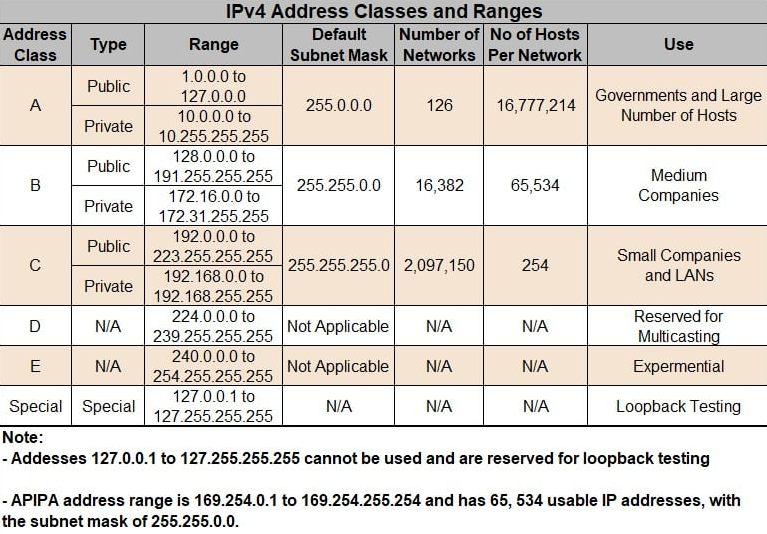
\includegraphics[width=0.8\textwidth]{images/ip_addresses.png}
    \caption{IP addresses types.}
    \label{fig:ip_address}
\end{figure}

\section{Operating Systems \& Programming Languages}
\lecture[4 hours]{03}{06}{2024}
A firewall is a crucial component in the realm of cybersecurity. It acts as a barrier that protects a network or system from external threats by managing and filtering incoming and outgoing network traffic. Essentially, a firewall serves as a gatekeeper between an internal network and the broader internet, analyzing network traffic and determining whether to allow or block data packets based on pre-established security rules.



\subsection{Key Classifications of Firewalls}

\begin{enumerate}
    \item \textbf{Firewall Types by Implementation:}
    \begin{itemize}
        \item \textbf{Hardware Firewalls:} These are physical devices dedicated to the task of network security. They are typically used by businesses and organizations with significant network traffic and complex security needs.

        \emph{Advantages}: high performance due to dedicated resources, capable of handling large volumes of traffic, centralized security management.

        \emph{Disadvantages}: higher cost and maintenance ,complexity in configuration and deployment.

        \item \textbf{Software Firewalls:} These are programs installed on individual computers or servers. They provide a flexible and often more economical solution, especially for personal use or smaller networks.

        \emph{Advantages}: cost-effective and easy to install, flexible and can be customized for specific needs, useful for personal devices and small businesses.

        \emph{Disadvantages}: consumes system resources, which can affect performance, requires individual management on each device.
    \end{itemize}

    \item \textbf{Firewall Placement:}
    \begin{itemize}
        \item \textbf{Perimeter Firewalls:} Positioned at the boundary of a network, perimeter firewalls are designed to safeguard the internal network from external threats. They act as the first line of defense, regulating access between the internal network and the internet or other untrusted networks.

        \emph{Advantages}: provides a robust first line of defense, centralized point of security control for the entire network.

        \emph{Disadvantages}: cannot protect against threats that bypass the perimeter, such as internal attacks.


        \item \textbf{Host-based Firewalls:} These are installed on individual devices within the network. They monitor and control traffic to and from the device on which they are installed, providing an additional layer of security.

        \emph{Advantages}: adds an extra layer of protection for individual devices, useful for controlling local traffic and internal threats.

        \emph{Disadvantages}: requires installation and management on each individual device, potentially increases the complexity of the overall security infrastructure.
    \end{itemize}
\end{enumerate}

\subsection{Types of traffic filtering}
Firewalls implement various types of traffic filtering to control which data packets can pass through or be blocked. Each type of firewall and filtering mechanism offers different levels of security and control over the network traffic.

\subsubsection{Static Packet Filtering}
Static packet filtering is a type of network traffic filtering where decisions to permit or block traffic are based on static criteria, such as IP addresses, source and destination ports, and protocols.

\begin{itemize}
    \item \textbf{Static Rules}: The firewall is configured with static rules created by the network administrator. These rules specify the criteria based on which the firewall evaluates the traffic.
    \item \textbf{Traffic Evaluation}: When the firewall receives a data packet, it compares the packet against the static rules. For example, it can check if the source and destination IP addresses are allowed, if the destination port is authorized, and if the protocol used is permitted.
    \item \textbf{Blocking or Permitting Decisions}: Based on these static rules, the firewall decides whether to permit or block the packet. If the packet matches the specified rules, it is allowed through; otherwise, it is blocked.
\end{itemize}

\subsubsection{Stateful Filtering}
Stateful filtering is an advanced type of filtering. Its distinguishing feature is the ability to track the state of network connections, enabling the firewall to make decisions based on contextual information about the connection.

\begin{itemize}
    \item \textbf{Initiated Connections}: A stateful firewall keeps track of connections initiated from the internal network and allows outgoing traffic associated with these connections.
    \item \textbf{Established Connections}: After detecting an initial connection, the stateful firewall maintains a list of established connections. This list contains information such as source and destination IP addresses, ports, and the current state of the connection.
    \item \textbf{Subsequent Packets}: When the firewall receives subsequent packets that are part of a previously established connection, it compares them with the connection information and decides whether to permit or block them. For example, if a packet is part of an established connection, it will usually be permitted.
\end{itemize}


\subsection{Web Application Firewall (WAF)}
A Web Application Firewall (WAF) is a cybersecurity component specifically designed to protect web applications from various online threats and attacks. This tool focuses on the application layer, analyzing incoming and outgoing web traffic to identify and block suspicious or dangerous activities.

\subsection{Next-Generation Firewall (NGFW)}

A Next-Generation Firewall (NGFW) is an advanced cybersecurity solution that combines traditional firewall functions with other advanced features and deep traffic inspection capabilities to provide more sophisticated protection against cyber threats.

\subsection{Proxy}

A proxy, or proxy server, is an intermediary server between a client (e.g., a computer or device) and a server the client wants to access. The proxy acts as a middleman between the client and the destination server, forwarding the client's requests and returning responses from the server.

\subsubsection{Functions of a Proxy}

\begin{itemize}
    \item \textbf{IP Address Hiding}: A proxy can hide the client's IP address from the destination server. When the client sends a request through the proxy, the proxy's IP address appears as the sender of the request to the server.
    \item \textbf{Content Filtering}: Some proxies are configured to filter traffic based on certain rules. For example, they can block access to specific websites or limit access to certain types of content.
    \item \textbf{Caching}: Proxies can locally store responses to client requests. This process allows the proxy to return responses to requests without having to forward them to the destination server, improving efficiency and speed.
    \item \textbf{Anonymity and Security}: Some proxies offer a degree of anonymity and security. For example, a proxy can hide the client's identity, making it more difficult for websites to track the user.
    \item \textbf{Remote Access}: Proxies can be used to allow remote access to internal network resources while protecting the security of the network.
\end{itemize}

\subsubsection{Reverse Proxy}
A reverse proxy is a type of proxy server that sits between client devices and a web server, handling requests from clients on behalf of the web server. It acts as an intermediary, forwarding client requests to the appropriate backend server and then returning the server's response to the client. Here is a detailed explanation of its functioning:

\begin{enumerate}
    \item \textbf{Client Request Handling}:
    \begin{itemize}
        \item When a client sends a request to access a web application or resource, the request is first received by the reverse proxy server instead of the actual web server.
        \item The client perceives the reverse proxy as the actual server, not knowing that their request is being handled by an intermediary.
    \end{itemize}

    \item \textbf{Request Forwarding}:
    \begin{itemize}
        \item The reverse proxy examines the client request and determines which backend server is best suited to handle the request. This determination can be based on various factors, such as load balancing policies, server health, or specific application logic.
        \item After identifying the appropriate backend server, the reverse proxy forwards the client request to this server.
    \end{itemize}

    \item \textbf{Response Handling}:
    \begin{itemize}
        \item Once the backend server processes the request, it sends the response back to the reverse proxy.
        \item The reverse proxy then sends this response to the client, making it appear as though the response originated from the reverse proxy itself.
    \end{itemize}

    \item \textbf{Load Balancing}:
    \begin{itemize}
        \item One of the key functions of a reverse proxy is to distribute incoming client requests across multiple backend servers to ensure no single server becomes overwhelmed with traffic. This process is known as load balancing.
        \item Load balancing can be implemented using various algorithms, such as round-robin, least connections, or IP hash, to effectively distribute the traffic load.
    \end{itemize}

    \item \textbf{Caching}:
    \begin{itemize}
        \item A reverse proxy can cache responses from backend servers. When subsequent requests for the same resource are received, the reverse proxy can serve the cached response instead of forwarding the request to the backend server, reducing latency and server load.
    \end{itemize}

    \item \textbf{SSL Termination}:
    \begin{itemize}
        \item Reverse proxies often handle SSL termination, which involves decrypting incoming SSL/TLS connections and forwarding the decrypted requests to the backend servers. This offloads the encryption/decryption overhead from the backend servers, improving their performance.
    \end{itemize}

    \item \textbf{Security and Anonymity}:
    \begin{itemize}
        \item Reverse proxies enhance security by hiding the identity and structure of the backend servers. Clients interact only with the reverse proxy, making it difficult for attackers to target the actual backend servers.
        \item They can also implement additional security measures such as Web Application Firewall (WAF) functionality, filtering malicious requests, and protecting backend servers from attacks.
    \end{itemize}

    \item \textbf{Compression}:
    \begin{itemize}
        \item Reverse proxies can compress responses from backend servers before sending them to clients. This reduces the amount of data transmitted over the network, improving load times and reducing bandwidth usage.
    \end{itemize}

    \item \textbf{Monitoring and Logging}:
    \begin{itemize}
        \item Reverse proxies can monitor and log traffic between clients and backend servers, providing valuable insights into performance, usage patterns, and potential security issues. These logs can be used for troubleshooting, capacity planning, and security auditing.
    \end{itemize}
\end{enumerate}

Overall, a reverse proxy acts as a mediator between clients and backend servers, enhancing performance, security, and scalability while simplifying the client-server interaction.

\subsection{Firewall Policies}

A firewall operates at various levels of the ISO/OSI model, providing diverse functionalities and security measures. The primary function of the firewall is to filter incoming or outgoing packets based on established rules known as firewall policies. These policies can filter packets based on:

\begin{itemize}
    \item \textbf{Source or Destination IP Address}
    \item \textbf{Destination Protocol or Port}
    \item \textbf{Geolocation} (origin of the request)
    \item \textbf{Application Used}
    \item \textbf{Type of Client}
\end{itemize}

When a firewall inspects a packet, it can decide how to handle it with the following actions:

\begin{itemize}
    \item \textbf{Allow}: The firewall lets the packet pass.
    \item \textbf{Drop}: The firewall discards the packet without sending any diagnostic message to the source.
    \item \textbf{Deny}: The firewall blocks the packet and informs the source.
\end{itemize}

These actions are specified in the firewall policies. For example, a policy might drop a packet directed to \texttt{google.com} on port 443 (HTTPS).

\subsubsection{Top-Down Policy Application}

Firewalls apply policies within the policy set using a top-down approach. For a given communication between a source and a destination, the firewall searches the policy set for a rule that manages the traffic. Once found, the firewall stops searching.

\begin{longtable}{|c|c|c|c|}
\hline
\textbf{Source IP} & \textbf{Destination IP} & \textbf{Port} & \textbf{Action} \\
\hline
192.168.1.15 & 10.10.10.10 & 443 & DENY \\ \hline
192.168.1.24 & 10.11.11.12 & 80, 53 & ACCEPT \\ \hline
192.168.23.40 & 10.10.11.11 & 0-1023 & ACCEPT \\\hline
192.168.23.40-41 & 192.168.33.54 & 443, 444, 445 & DENY \\\hline
10.10.10.0/24 & Group-ip-microsoft & 443, 1234, 998 & DROP \\\hline
Object-google-ip & 10.10.10.0/24 & High-ports-group & DENY \\\hline
ANY & ANY & ANY & DENY \\
\hline
\end{longtable}

\paragraph{Policy Evaluation Example}

Consider the following example:

\begin{itemize}
    \item The firewall intercepts a flow and examines the policy set to determine the appropriate action.
    \item It first checks the policy set's top rule. If it doesn't match the flow, the firewall moves to the next rule.
    \item If the third rule includes the traffic flow, the firewall handles the flow according to the "ACTION" parameter, allowing the traffic to pass ("ACCEPT").
\end{itemize}

\subsubsection{Source and Destination IP Fields}

The source and destination IP fields can include:
\begin{itemize}
    \item Multiple IP addresses
    \item Subnets
    \item Groups / Objects
\end{itemize}

If the firewall does not find any rules that manage the flow, it discards the flow using a default rule. This rule, present in all policy sets and not modifiable, rejects all communications that do not match any other rule.

\subsubsection{Default Rule Scenario}

\textbf{What happens if this default policy is placed at the top of the policy set?}

If the default deny rule is the first rule evaluated by the firewall, all traffic will be blocked because it matches the "ANY ANY ANY DENY" rule. This setup would effectively prevent all communications through the firewall.


\subsection{Intrusion Detection and Prevention Systems}

\subsubsection{Intrusion Detection System (IDS)}

An Intrusion Detection System (IDS) is a cybersecurity tool designed to detect and report suspicious activities or intrusions in networks or computer systems. It continuously monitors network traffic, system logs, and other events to identify anomalies that may indicate a security threat.

\begin{itemize}
    \item \textbf{Traffic Analysis}: IDS analyzes network traffic or system logs to identify known attack signatures, anomalous behaviors, or policy violations.
    \item \textbf{Alert Generation}: When a potential threat is detected, IDS generates alerts or notifications for security administrators to take appropriate actions.
    \item \textbf{Passive System}: IDS does not take direct action to stop an attack; it only provides alerts.
\end{itemize}

\subsubsection{Intrusion Prevention System (IPS)}

An Intrusion Prevention System (IPS) is a cybersecurity tool that, unlike an IDS, can take active measures to block or prevent detected attacks. IPS operates in real-time to immediately interrupt malicious or unwanted activities.

\begin{itemize}
    \item \textbf{Real-Time Response}: IPS not only detects threats but also takes proactive actions to stop them, such as blocking suspicious traffic or disconnecting users.
    \item \textbf{Preventive Actions}: When a threat is detected, IPS can block traffic, issue alerts, or take other actions to prevent the attack from causing damage.
    \item \textbf{Active System}: The primary goal of IPS is to prevent cyber attacks from harming the system or network before any damage occurs. However, careful configuration is required to avoid false positives, which could block legitimate traffic.
\end{itemize}

\subsection{Network Zoning for Enhanced Security}

After discussing some network security devices, let's explore a commonly used technique to significantly enhance network security: zoning. This technique involves dividing the network into different zones.

\subsubsection{Principle of Zoning}

\begin{itemize}
    \item \textbf{Application Area}: A zone dedicated to applications.
    \item \textbf{User PCs Area}: A zone dedicated to user PCs.
    \item \textbf{Admin PCs Area}: A zone dedicated to administrators' PCs.
\end{itemize}

Clearly, a network can have areas or zones that require higher levels of security due to their sensitivity.

\subsubsection{Zoning Implementation}

\begin{itemize}
    \item \textbf{Segregation}: Networks are segmented into zones based on asset criticality and the required security level.
    \item \textbf{Security Levels}: Different zones have varying security measures, ensuring that sensitive areas have stricter controls.
\end{itemize}

\subsection{Multi-Tier DMZ Structure}

Cyber threats primarily originate from the internet, prompting many organizations to implement a multi-tier DMZ (Demilitarized Zone) network structure. This setup involves:

\subsubsection{Multi-Tier DMZ Structure}

\begin{itemize}
    \item \textbf{Zone Division}: The network is divided into zones based on the criticality of assets on each segment.
    \item \textbf{Multiple Security Layers}: Additional security layers, such as firewalls, proxies, or other security devices, are added.
\end{itemize}


\subsection{Encryption: Meaning and Types}

\subsubsection{What Does Encryption Mean?}

Encryption refers to the process of converting data or a message into an unreadable or unintelligible format unless one possesses a specific key or method to decrypt it. The main goal of encryption is to protect sensitive or confidential information, making it inaccessible to unauthorized individuals. Encryption can be used for various purposes, including:

\begin{itemize}
    \item \textbf{Communication Security}: To protect the privacy of online communications, such as during financial transactions or instant messaging, ensuring that only the authorized sender and recipient can read the message.
    \item \textbf{Data Storage Protection}: To secure data stored on devices like hard drives, USB flash drives, or servers, so that if someone physically accesses the data, they cannot read it without the correct access key.
    \item \textbf{Authentication and Digital Signatures}: To verify the authenticity of messages or digital documents and ensure they have not been altered during transmission or storage.
    \item \textbf{Protection of Trade Secrets}: In businesses, encryption is often used to protect trade secrets, customer data, and other sensitive information.
\end{itemize}

\subsubsection{Main Approaches in Modern Encryption}

There are two main approaches in modern computer encryption: symmetric key encryption and asymmetric key encryption.

\paragraph{Symmetric Key Encryption}

Symmetric key encryption is like a lock with a single key. Both the sender and recipient share the same secret key to encrypt and decrypt the data.

\begin{itemize}
    \item \textbf{Encryption Process}: The sender uses the secret key to transform plaintext into an unreadable format.
    \item \textbf{Decryption Process}: The recipient uses the same secret key to decrypt the message and restore it to its original form.
    \item \textbf{Efficiency}: This method is fast and efficient but requires secure key management.
\end{itemize}

Symmetric Key Encryption Example Using AES:

\begin{enumerate}
    \item \textbf{Preparation}:
    \begin{itemize}
        \item \textbf{Plaintext Message}: "HELLO WORLD!"
        \item \textbf{Secret Key}: "SECRETKEY123456"
    \end{itemize}

    \item \textbf{Encryption Process}:
    \begin{itemize}
        \item \textbf{Algorithm}: AES uses multiple rounds of substitution, permutation, and combination.
        \item \textbf{Combination}: Plaintext and secret key are combined through several rounds to generate ciphertext.
        \item \textbf{Result}: Ciphertext is a seemingly random sequence of data.
    \end{itemize}

    \item \textbf{Decryption Process}:
    \begin{itemize}
        \item \textbf{Secret Key}: The same key used for encryption.
        \item \textbf{Inverse Operations}: AES performs the inverse operations to restore plaintext from ciphertext.
        \item \textbf{Decrypted Message}: The original message "HELLO WORLD!" is obtained.
    \end{itemize}
\end{enumerate}



\paragraph{Asymmetric Key Encryption (Public/Private Key Encryption)}

Asymmetric key encryption, also known as public/private key encryption, involves two distinct keys that work complementarily to encrypt and decrypt data.

\begin{itemize}
    \item \textbf{Public Key}:
    \begin{itemize}
        \item Available publicly and can be distributed widely.
        \item Each user has their own public key, which can be freely shared with others.
        \item Used to encrypt data before sending it to a recipient.
    \end{itemize}

    \item \textbf{Private Key}:
    \begin{itemize}
        \item Kept secret and known only to the owner.
        \item Used to decrypt data encrypted with the corresponding public key.
    \end{itemize}

    \item \textbf{Digital Signatures}:
    \begin{itemize}
        \item Used to create digital signatures, serving as an "electronic seal" that verifies the sender's authenticity and the integrity of the data.
        \item The process includes key pair generation, document hashing, signing, and verification, as shown in \Cref{fig:digital_sign}.

        \begin{figure}[h!]
            \begin{center}
                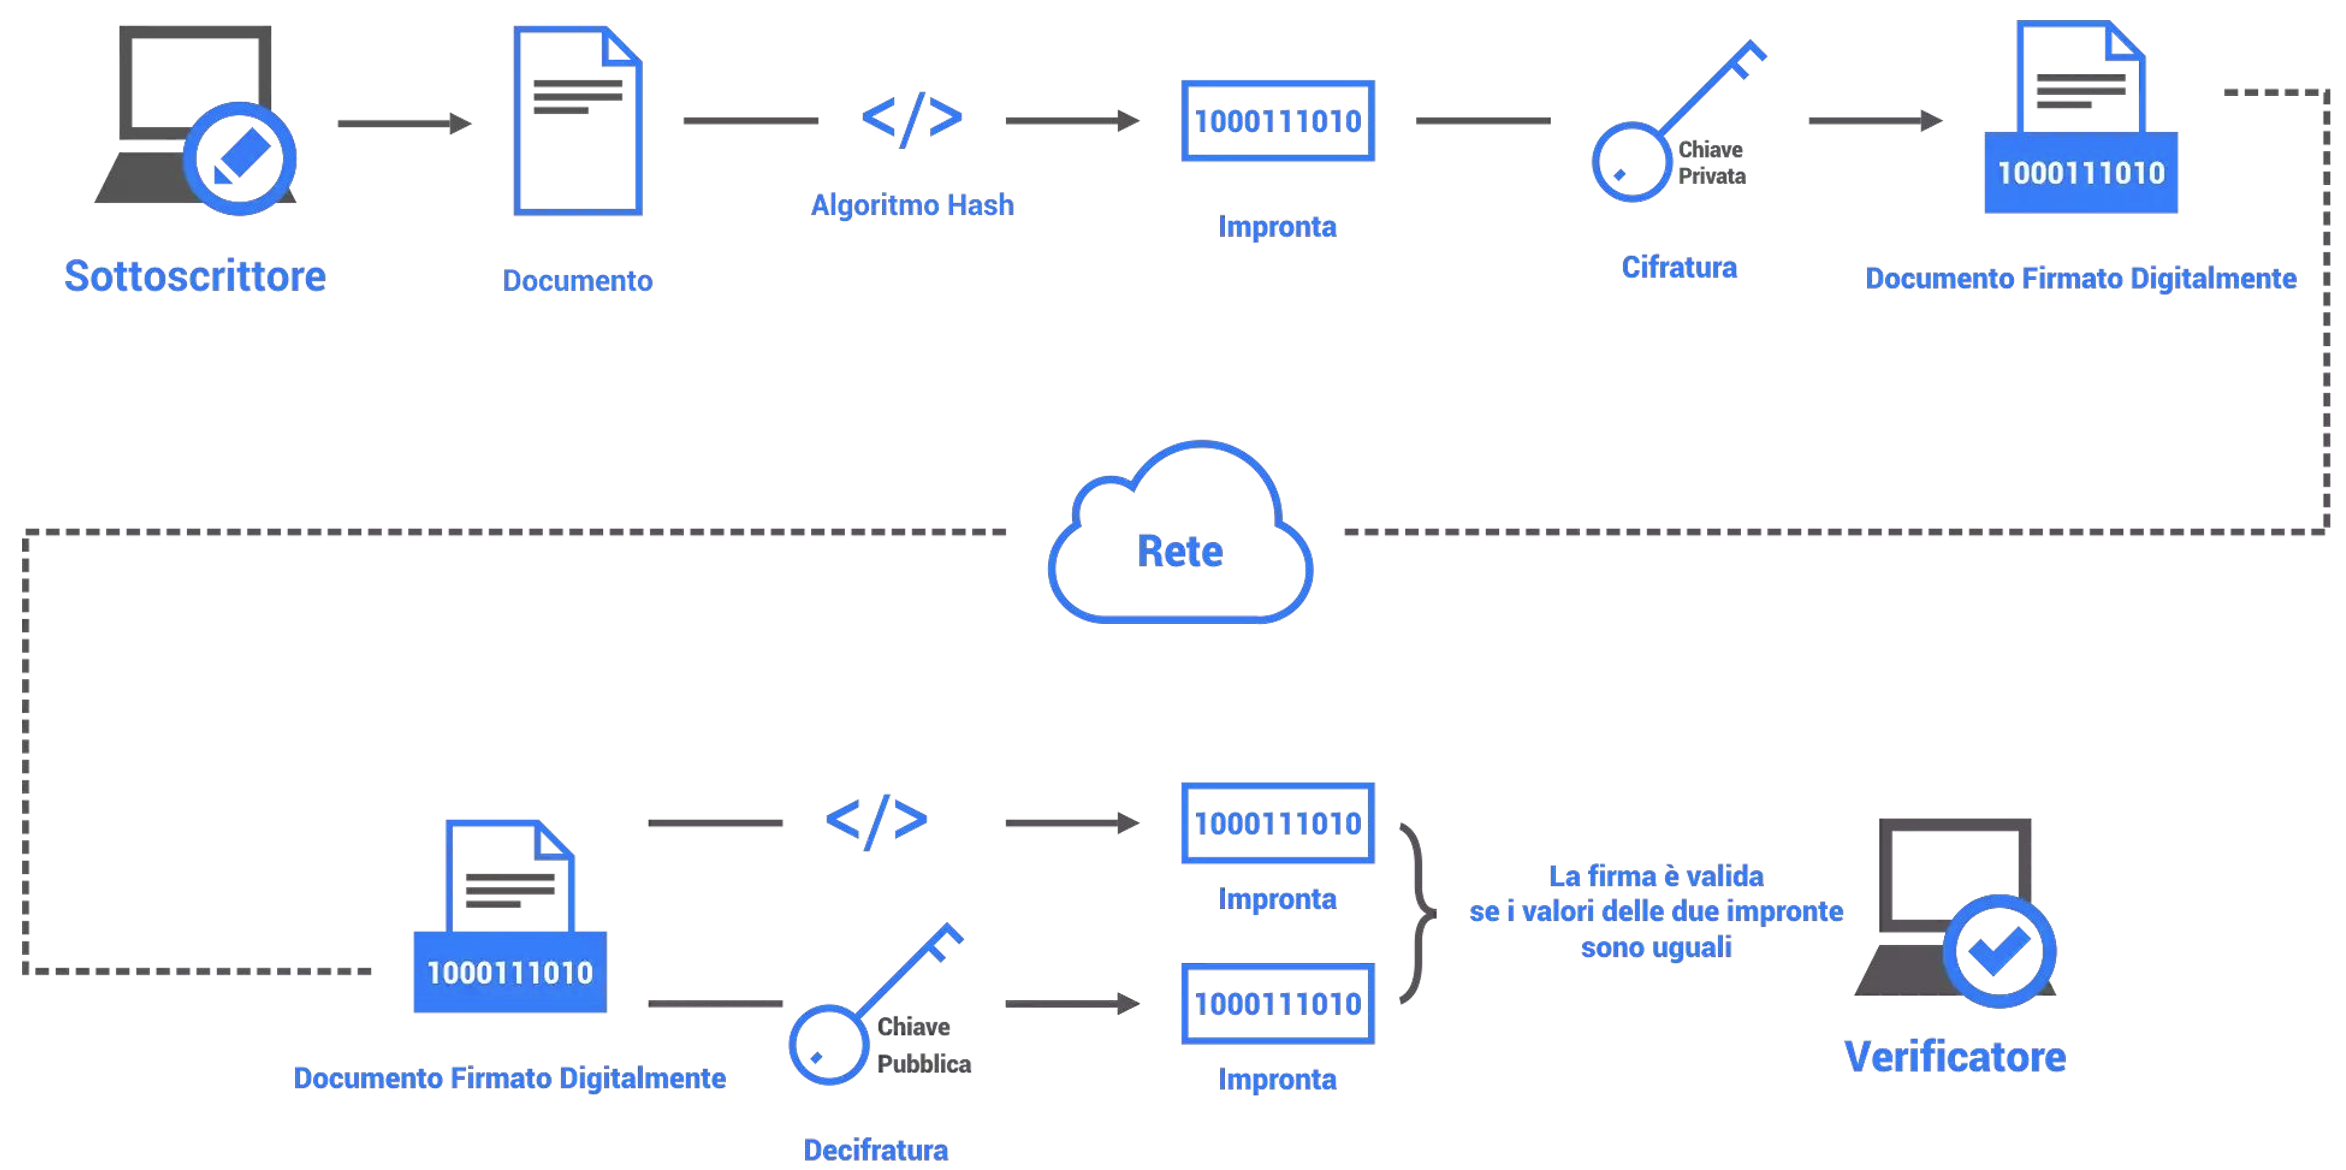
\includegraphics[width=\textwidth]{images/digital_sign.png}
                \caption{Digital signature schematics.}
                \label{fig:digital_sign}
            \end{center}
        \end{figure}
    \end{itemize}

\end{itemize}

\subsection{What Is a VPN?}

A VPN, or Virtual Private Network, is a technology that creates a secure connection over the internet between your device and a remote server or between two devices.

\subsubsection{Main Functions of a VPN}

\begin{itemize}
    \item \textbf{Security}: Encrypts traffic between your device and the VPN server, ensuring intercepted data cannot be read or interpreted.
    \item \textbf{Privacy}: Hides your real IP address and geographic location, making it difficult for websites and online services to track your activity or location.
    \item \textbf{Access to Geo-Blocked Resources}: Allows you to choose a VPN server, enabling you to bypass geographic restrictions.
    \item \textbf{Public Network Security}: Protects you from potential attacks when connected to public Wi-Fi networks, such as in cafes or airports.
\end{itemize}


\section{Python for Hackers and Web Applications}

\section{BUILD WEEK 1: Network Security design}

\section{Operating Systems}

\subsection{Microsoft Windows}
Microsoft Windows, commonly referred to as Windows, is a family of graphical operating systems developed, marketed, and sold by Microsoft Corporation since 1985. It is designed for use on personal computers, workstations, servers, and smartphones. The name "Windows" originates from the window-based graphical user interface (GUI) known as File Explorer. Windows is a multitasking operating system, meaning it can run multiple programs simultaneously. From its inception, Windows has been conceived as a graphical operating system, implementing the "desktop metaphor" with icons, buttons, backgrounds, taskbars, status bars, and many other features.

\subsubsection{Windows Shell and PowerShell}
The shell, or command interpreter, is a program that allows interaction with the operating system via a terminal and command-line interface. Windows PowerShell is an advanced shell integrated into all Microsoft operating systems starting from Windows 7. It includes an interactive prompt and a scripting environment that can be used separately or in combination. PowerShell is a command-line shell designed specifically for system administrators, offering extensive scripting capabilities to automate routine tasks. Key features and advantages of PowerShell include:
\begin{itemize}
    \item \textbf{Integration with Microsoft .NET}: PowerShell leverages the .NET framework, providing extensive functionality through reusable libraries and functions.
    \item \textbf{Object-Oriented}: Unlike traditional shells that return plain text, PowerShell returns objects, enabling more complex data manipulation.
    \item \textbf{Command-Lets (cmdlets)}: PowerShell commands are structured as verb-noun pairs, facilitating intuitive command usage.
    \item \textbf{Admin-Oriented}: PowerShell includes features designed for system administrators, such as remote management and the ability to perform administrative tasks.
\end{itemize}

\subsubsection{Common PowerShell Cmdlets}
One of PowerShell's strengths is its cmdlets, which are structured as a verb followed by a noun. To display the complete set of available cmdlets, the \texttt{Get-Command} cmdlet can be used. PowerShell allows the use of the pipe operator (|) to chain multiple cmdlets, using the output of one cmdlet as the input for the next. This technique is particularly useful for text processing tasks.

\begin{table}[h!]
    \centering
    \begin{adjustbox}{width=1\textwidth}
    \begin{tabular}{|c|c|c|}
    \hline
    \textbf{Cmdlet} & \textbf{Aliases} & \textbf{Description} \\
    \hline
    \texttt{Set-Location} & cd, chdir, sl & Sets the current working location to a specified location. \\
    \texttt{Get-Content} & cat, gc, type & Gets the content of the item at the specified location. \\
    \texttt{Add-Content} & ac & Adds content to the specified items, such as adding words to a file. \\
    \texttt{Set-Content} & sc & Writes or replaces the content in an item with new content. \\
    \texttt{Copy-Item} & copy, cp, cpi & Copies an item from one location to another. \\
    \texttt{Remove-Item} & del, erase, rd, ri, rm, rmdir & Deletes the specified items. \\
    \texttt{Move-Item} & mi, move, mv & Moves an item from one location to another. \\
    \texttt{Set-Item} & si & Changes the value of an item to the value specified in the command. \\
    \texttt{New-Item} & ni & Creates a new item. \\
    \texttt{Start-Job} & sajb & Starts a Windows PowerShell background job. \\
    \texttt{Compare-Object} & compare, dif & Compares two sets of objects. \\
    \texttt{Group-Object} & group & Groups objects that contain the same value for specified properties. \\
    \hline
    \end{tabular}
\end{adjustbox}
    \caption{Common PowerShell Cmdlets}
    \label{table:cmdlets}
    \end{table}

    \begin{table}[h!]
    \centering
    \begin{adjustbox}{width=1\textwidth}
    \begin{tabular}{|c|c|c|}
    \hline
    \textbf{Cmdlet} & \textbf{Aliases} & \textbf{Description} \\
    \hline
    \texttt{Invoke-WebRequest} & curl, iwr, wget & Gets content from a web page on the Internet. \\
    \texttt{Measure-Object} & measure & Calculates numeric properties of objects, and the characters, words, and lines in string objects. \\
    \texttt{Resolve-Path} & rvpa & Resolves the wildcard characters in a path and displays the path contents. \\
    \texttt{Resume-Job} & rujb & Restarts a suspended job. \\
    \texttt{Set-Variable} & set, sv & Sets the value of a variable. Creates the variable if one with the requested name does not exist. \\
    \texttt{Show-Command} & shcm & Creates Windows PowerShell commands in a graphical command window. \\
    \texttt{Sort-Object} & sort & Sorts objects by property values. \\
    \texttt{Start-Service} & sasv & Starts one or more stopped services. \\
    \texttt{Start-Process} & saps, start & Starts one or more processes on the local computer. \\
    \texttt{Suspend-Job} & sujb & Temporarily stops workflow jobs. \\
    \texttt{Wait-Job} & wjb & Suppresses the command prompt until one or all of the Windows PowerShell background jobs running in the session are complete. \\
    \texttt{Where-Object} & ?, where & Selects objects from a collection based on their property values. \\
    \hline
    \end{tabular}
    \end{adjustbox}
    \caption{Additional PowerShell Cmdlets}
    \label{table:cmdlets2}
    \end{table}

\subsubsection{Windows File System}
The Windows file system is an organizational structure within the operating system that regulates the naming, storage, and retrieval of files. PowerShell provides cmdlets to interact with the file system, files, and directories.

\begin{itemize}
    \item \texttt{Get-ChildItem}: Displays the contents of a directory.
    \item \texttt{Copy-Item}: Copies a file from one location to another. This cmdlet accepts two parameters: the source file and the destination.
\end{itemize}

\subsubsection{Components of Windows Operating System}
The fundamental components of the Windows operating system are depicted in the diagram (Figure~\ref{fig:components}). Windows OS distinguishes between user space and kernel space as a security measure, separating tasks that require special privileges from those that do not. The DLL (Dynamic Link Library) subsystems interface between kernel mode and user mode, providing function libraries that users and applications can utilize to request the kernel to perform specific tasks.

\begin{figure}[h!]
\centering
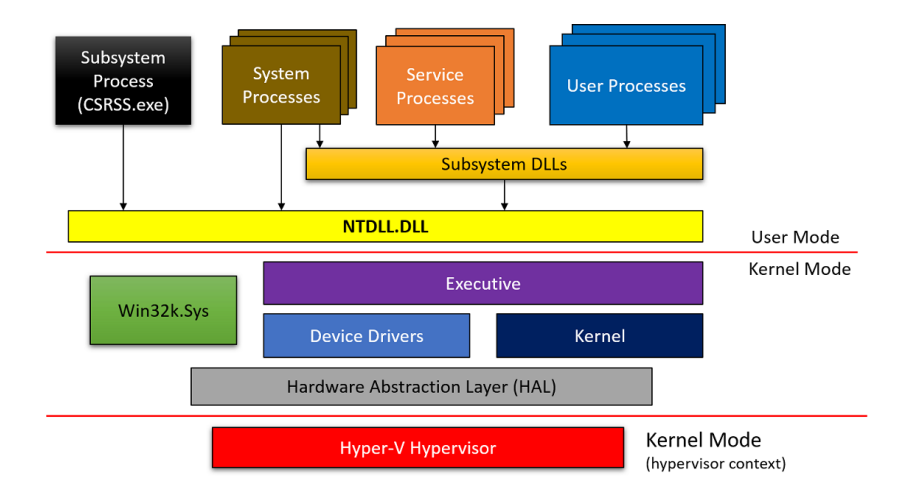
\includegraphics[width=0.8\textwidth]{images/user_kernel.png}
\caption{Components of Microsoft Windows Operating System}
\label{fig:components}
\end{figure}

\begin{itemize}
    \item User Applications: User applications run in user mode and can be either 32-bit or 64-bit, depending on the operating system.
    \item Services: This includes active processes and services in Windows, such as the task manager or network services.
    \item Executive: The executive contains the core functionalities of the operating system, including memory management, security features, and process management.
    \item Driver Management: Manages calls to input/output devices.
    \item Kernel: The kernel encompasses low-level OS functions, such as thread scheduling, interrupts, exception handling, and multiprocessor synchronization.
\end{itemize}



\subsubsection{Windows Hybrid Kernel}
The Windows kernel is a hybrid kernel, meaning it incorporates elements of both monolithic and microkernel architectures.

\begin{itemize}
    \item Monolithic Kernel: A monolithic kernel runs most operations directly in kernel space, including memory management, process management, and system calls, providing high performance but potentially lower stability due to the lack of isolation between components.
    \item Microkernel: A microkernel, conversely, delegates many functionalities to user space processes, keeping only essential functions in the kernel, which enhances modularity and stability at the cost of potential performance overhead due to increased inter-process communication.
    \item Hybrid Kernel: Windows hybrid kernel aims to balance the speed of a monolithic kernel with the modularity and stability of a microkernel by implementing critical functions within the kernel and allowing certain components, such as device drivers, to run in user space.
\end{itemize}


\subsection{Linux Operating Systems}
The origins of the Unix Operating System date back to the late 1960s with the development of the MULTICS (Multiplexed Information and Computing Service) project. This project was a collaboration between AT\&T, Honeywell, General Electric, and the Massachusetts Institute of Technology (MIT), sponsored by ARPA, the research arm of the U.S. Department of Defense. The goal was to create an operating system capable of continuing to function even if some parts of the computer were shut down or deactivated, thereby not affecting the work of users utilizing the still-active components. The modularity of this system allowed for improvements or expansions by simply adding new modules, without the need to rebuild the entire system from scratch.

In 1991, Linus Torvalds, a computer science student from Helsinki, released a version of the Minix monolithic kernel that could run on a standard Intel 386 processor, and he distributed it freely along with its source code. This project evolved into what we now know as the Linux kernel, which has been periodically updated and revised over the years.

Today, Linux is one of the most widely used operating systems for:
\begin{itemize}
    \item Web Servers
    \item High-performance applications
    \item Embedded systems
    \item Network systems
\end{itemize}
Linux is freely distributed, meaning that all users can download it and contribute to the project. The term "free software" was initially popularized by Richard Stallman, emphasizing that users are granted the following rights:
\begin{itemize}
    \item The freedom to run the program
    \item The freedom to study how the program works
    \item The freedom to redistribute copies of the program
    \item The freedom to modify the program
\end{itemize}

\subsubsection{Structure of the Linux Operating System}
As an operating system, Linux serves as an interface between the user and the machine, providing a set of tools and functionalities. The primary components are:
\begin{itemize}
    \item Hardware
    \item Operating System
    \item Shell
    \item GUI (Graphical User Interface)
    \item Applications
\end{itemize}
The operating system sits between the hardware and user applications, providing routines for managing processes, memory, and other resources. This type of kernel is known as a "monolithic" kernel.

\subsubsection{Types of Kernels}
There are several types of kernels used in operating systems:
\begin{itemize}
    \item \textbf{Microkernel}: A minimalistic kernel that includes only the basic functionalities required for the operating system to function. An example is MINIX.
    \item \textbf{Monolithic Kernel}: A single binary file that includes most of the operating system's functionalities. An example is the Unix kernel.
    \item \textbf{Modular Kernel}: An extension of the monolithic kernel, capable of adding or removing modules as needed.
\end{itemize}

\begin{figure}[h!]
\centering
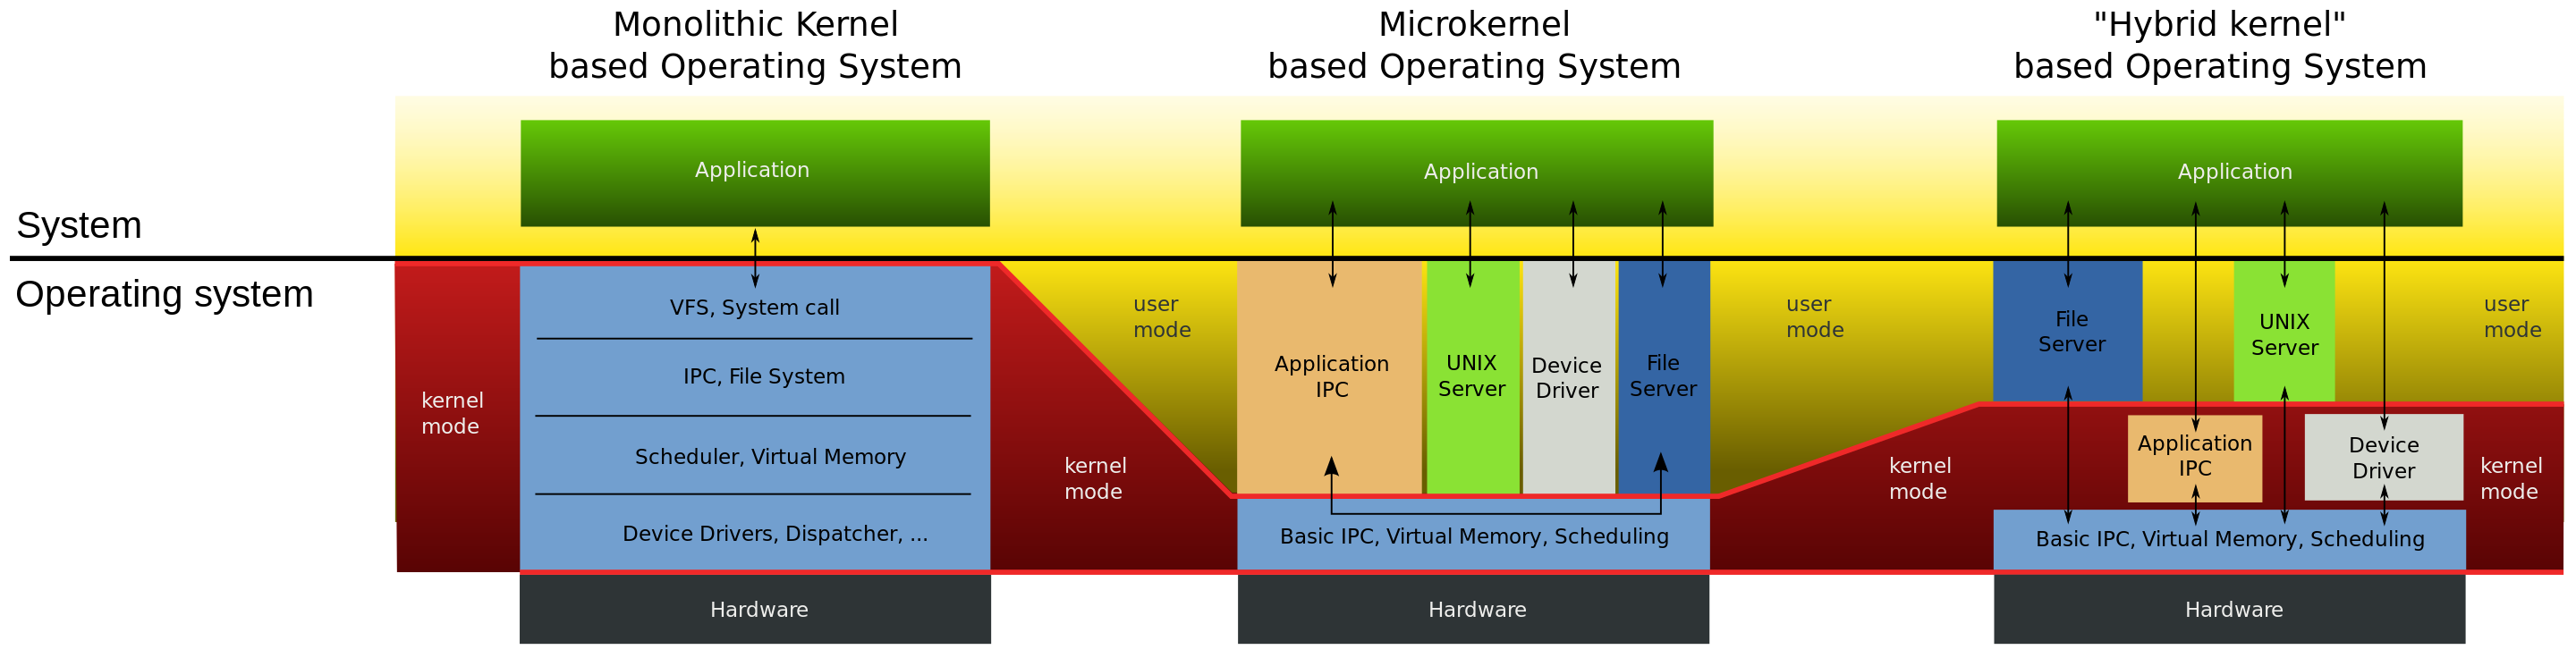
\includegraphics[width=\textwidth]{images/kernels.png}
\caption{Types of Kernels: Microkernel, Modular, Monolithic}
\label{fig:kernels}
\end{figure}

\subsubsection{Processes in Linux}
In Linux, a process is an instance of a program in execution, assigned to a processor for instruction execution. A process has a state, which is read by the CPU for scheduling and process switching. Linux processes are complex structures characterized by:
\begin{itemize}
    \item Memory addresses used
    \item Content of the addressed memory
    \item Pointers to input/output devices used
    \item Data, i.e., variables used by the process
    \item Threads
\end{itemize}

\paragraph{Threads}
Threads are tasks within a process. A process can perform various functions using multiple threads, each handling separate tasks. Threads within a process share the same state and memory information, allowing independent action on the used resources. Proper prioritization by the operating system is crucial to avoid simultaneous modification of the same resource by different threads (synchronization issue).

In Linux, each process is identified by a Process Identifier (PID), while each thread within a process is identified by a Thread Identifier (TID). Processes are created by invoking the system call \texttt{Fork()}. The child process created with \texttt{Fork()} inherits attributes from the parent process.

\begin{table}[h!]
\centering
\begin{tabular}{|c|c|}
\hline
\textbf{Command} & \textbf{Description} \\
\hline
\texttt{mkdir} & Creates a directory \\
\texttt{rmdir} & Removes a directory \\
\texttt{cp} & Copies files and directories \\
\texttt{rm} & Removes files \\
\texttt{mv} & Moves or renames files \\
\texttt{ls} & Lists directory contents \\
\texttt{cd} & Changes the current directory \\
\hline
\end{tabular}
\caption{Common Linux File System Commands}
\label{table:filesystem_commands}
\end{table}

\subsubsection{Linux File System}
The Linux file system originates in the root directory, denoted as \texttt{/}. The root user, or system administrator, has extensive control over the system. Key directories in the Linux file system include:
\begin{itemize}
    \item \texttt{/bin}: Contains essential system programs available for booting the system.
    \item \texttt{/home}: Contains user-specific directories and files.
    \item \texttt{/usr}: Contains installed programs, manual files, and documentation.
    \item \texttt{/sbin}: Similar to \texttt{/bin} but for system administration.
    \item \texttt{/etc}: Contains system and application configuration files.
\end{itemize}

\subsubsection{User Management in Linux}
Linux systems often support multiple users, necessitating mechanisms to separate user data and protect privacy. Each user is assigned a unique user identifier (UID) and a home directory. File permissions ensure that private files are not accessible to other users. User information is stored in \texttt{/etc/passwd}, which includes:
\begin{itemize}
    \item Group IDs
    \item User IDs
    \item Login shell
    \item Encrypted password (hashed)
\end{itemize}

Linux, with its rich history and robust architecture, continues to be a cornerstone in modern computing. Its versatility, security, and open-source nature make it a preferred choice for servers, high-performance applications, embedded systems, and network systems.

\section{Programming Languages}
\subsection{Introduction}
Becoming an Ethical Hacker necessitates a profound understanding of various programming languages. Many hacking tools are custom-developed by hackers themselves, thus, a solid foundation in key programming languages is essential. This document explores some of the fundamental programming languages used in cybersecurity, particularly focusing on:

\begin{itemize}
    \item \textbf{C Language} is considered the foundation of many programming languages, with most libraries and Linux code written in C.
    \item \textbf{Python Language}, an interpreted, object-oriented language, is widely used by hackers due to its simplicity and effectiveness.
\end{itemize}

\subsubsection{Classification of Programming Languages}
Today, there are innumerable programming languages, which can be categorized into the following traditional classifications:
\begin{itemize}
    \item Machine Languages: in machine language, algorithms are encoded using binary code, often referred to as "words" of 0s and 1s (bits). The computer directly executes instructions written in machine language.
    \item Assembly Languages: assembly language defines a set of elementary operations using a more human-readable syntax. This language is closer to human language but still requires a translator (assembler) for the computer to execute the code.
    \item High-Level Languages: high-level programming languages are much closer to human languages. Their instructions are comprehensible and easy to use. However, they also require a translator (compiler or interpreter) to convert high-level language into machine language (sequences of 0s and 1s).
\end{itemize}

\subsubsection{Types of Translators}
There are two primary types of translators:
\begin{itemize}
    \item Compiler: Translates a program written in a high-level language into machine language.
    \item Interpreter: Analyzes and translates a program written in a high-level language and executes the instructions simultaneously.
\end{itemize}

\subsubsection{Error Types in Programming}
When programming, it is beneficial to understand the types of errors that might be encountered. Programming errors can be divided into three categories:
\begin{itemize}
    \item Syntax Errors: Syntax errors are typographical mistakes made during the coding phase. These are the easiest to resolve as compilers often indicate the location of the error by providing the line number where the error occurred.
    \item Logical Errors: Logical errors occur during the design phase of the algorithm. These are more challenging to fix because the compiler does not identify them; the program will still compile successfully.
    \item Runtime Errors: Runtime errors occur post-compilation when the program is running. These are difficult to identify as they are not detected by the compiler.
\end{itemize}


\subsection{C Programming Language}

The C programming language is a general-purpose, procedural computer programming language that was developed in the early 1970s by Dennis Ritchie at Bell Labs. It has since become one of the most widely used programming languages of all time due to its efficiency, portability, and flexibility.

\subsubsection{Main Properties of C Language}
\begin{itemize}
    \item \textbf{Low-Level Access}: C provides low-level access to memory through pointers, making it ideal for system programming.
    \item \textbf{Portability}: C programs can be compiled and run on various computer systems with minimal or no modification.
    \item \textbf{Rich Library}: The Standard C Library provides numerous built-in functions for performing input/output, string manipulation, memory allocation, and more.
    \item \textbf{Modularity}: C supports modular programming through the use of functions, allowing code to be organized and reused.
    \item \textbf{Structured Language}: C allows complex programs to be broken into simpler subprograms or functions, facilitating easier management and debugging.
\end{itemize}

\section{Basic Syntax and Commands in C}
\subsection{Data Types}
C supports several built-in data types, which can be categorized as follows:

\begin{table}[h!]
\centering
\begin{tabular}{|c|c|c|}
\hline
\textbf{Data Type} & \textbf{Description} & \textbf{Size (bytes)} \\
\hline
\texttt{int} & Integer & 2 or 4 \\
\texttt{float} & Floating point & 4 \\
\texttt{double} & Double precision floating point & 8 \\
\texttt{char} & Character & 1 \\
\texttt{void} & Empty type & 0 \\
\hline
\end{tabular}
\caption{Basic Data Types in C}
\label{table:data_types}
\end{table}

\subsubsection{Control Structures}
C provides several control structures for directing the flow of a program:

\begin{itemize}
    \item \textbf{Conditional Statements}
        \begin{itemize}
            \item \texttt{if}, \texttt{else if}, \texttt{else}
            \item \texttt{switch}, \texttt{case}, \texttt{default}
        \end{itemize}
    \item \textbf{Loops}
        \begin{itemize}
            \item \texttt{for} loop
            \item \texttt{while} loop
            \item \texttt{do-while} loop
        \end{itemize}
    \item \textbf{Jump Statements}
        \begin{itemize}
            \item \texttt{break}
            \item \texttt{continue}
            \item \texttt{return}
            \item \texttt{goto}
        \end{itemize}
\end{itemize}

\subsubsection{Functions}
Functions in C are used to modularize code. The general form of a function definition is:

\begin{verbatim}
return_type function_name(parameters) {
    // body of the function
}
\end{verbatim}

\begin{table}[h!]
\centering
\begin{tabular}{|c|c|}
\hline
\textbf{Keyword} & \textbf{Description} \\
\hline
\texttt{void} & Specifies that the function does not return a value \\
\texttt{int} & Specifies that the function returns an integer value \\
\texttt{float} & Specifies that the function returns a floating-point value \\
\texttt{char} & Specifies that the function returns a character value \\
\hline
\end{tabular}
\caption{Common Function Return Types in C}
\label{table:function_return_types}
\end{table}

\subsubsection{Input/Output Operations}
C uses the Standard Input and Output library (\texttt{stdio.h}) for input and output operations. The most commonly used functions are:

\begin{table}[h!]
\centering
\begin{tabular}{|c|c|}
\hline
\textbf{Function} & \textbf{Description} \\
\hline
\texttt{printf()} & Prints formatted output to the console \\
\texttt{scanf()} & Reads formatted input from the console \\
\texttt{getchar()} & Reads a single character from the console \\
\texttt{putchar()} & Writes a single character to the console \\
\texttt{fgets()} & Reads a string from a file or the console \\
\texttt{fputs()} & Writes a string to a file or the console \\
\hline
\end{tabular}
\caption{Common Input/Output Functions in C}
\label{table:io_functions}
\end{table}

The C programming language is foundational to many other programming languages and is extensively used in system and application software, embedded systems, and high-performance server and client applications. Its efficiency, portability, and modularity make it a valuable language to learn for aspiring ethical hackers and cybersecurity professionals.

\section{Understanding Pointers, Memory Management, Stacks, and Arrays in C}

\subsection{Pointers}
Pointers are a type of variable that contain memory addresses. A pointer in C is declared by prefixing the variable name with an asterisk (\texttt{*}). For example:
\begin{lstlisting}
int *i; // pointer to an integer
char *c; // pointer to a character
\end{lstlisting}

There are two main operations that can be performed with a pointer:
\begin{itemize}
    \item Change the content at the memory address the pointer points to.
    \item Change the address that the pointer points to.
\end{itemize}

\noindent Consider the following example:
\begin{lstlisting}
int var = 123;
int *i;
i = &var; // pointer i points to the address of var
*i = 5;  // the content at the address pointed by i is changed to 5
\end{lstlisting}

After execution, \texttt{var} will be 5.

\begin{figure}[h!]
    \centering
    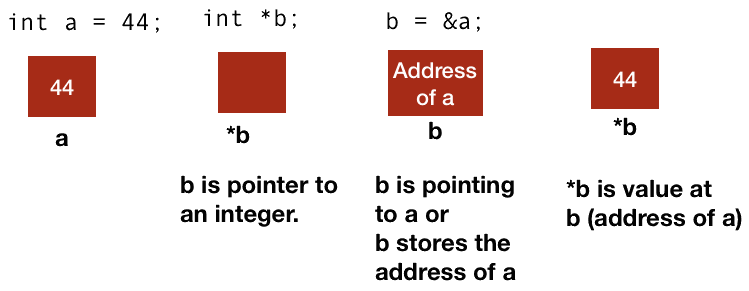
\includegraphics[width=0.8\textwidth]{images/pointers_c.png}
    \caption{Pointers in C.}
\end{figure}

\subsection{Memory Management in C}
During the execution of a program, memory in C is managed in two ways:
\begin{itemize}
    \item \textbf{Static Memory Management}: A fixed memory area is allocated by the operating system for the entire duration of the program.
    \item \textbf{Dynamic Memory Management}: Two distinct memory areas are allocated and used as needed: the stack and the heap.
\end{itemize}

\subsubsection{Stack}
The stack in C is a special region of a program's memory that stores temporary variables created by each function (including the \texttt{main} function). It plays a crucial role in managing function calls, local variables, and control flow.
The stack is used for variables and function parameters. For each function call, a new stack frame is created with its parameters. When the function completes, its stack frame is removed, and the stack reverts to its previous state. The stack operates on the Last In, First Out (LIFO) principle. This means that the last item pushed onto the stack is the first one to be popped off. Think of it like a stack of plates: you can only add or remove the top plate.

\begin{figure}[h!]
    \centering
    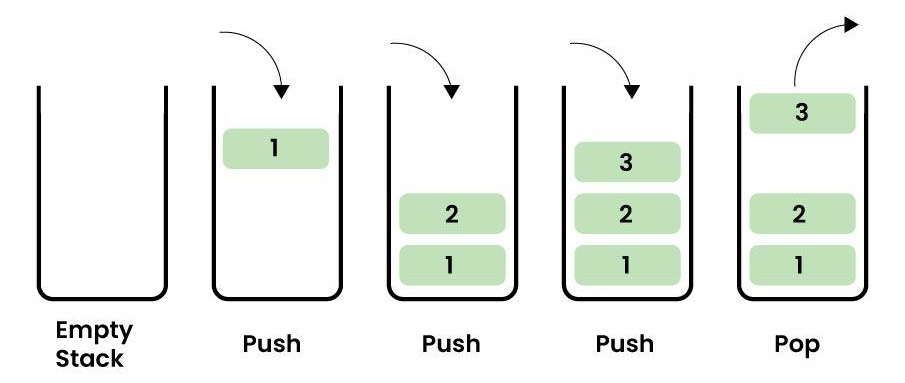
\includegraphics[width=0.8\textwidth]{images/lifo.jpg}
\end{figure}

\paragraph{Heap}
The heap is a memory area managed by the programmer and can be dynamically allocated as needed using C's memory management libraries.

\begin{itemize}
    \item The \textbf{ESP} (Extended Stack Pointer) register points to the top of the current stack frame. It keeps track of the last used location in the stack. When a function is called, the ESP is adjusted to allocate space for the function's local variables. When a function returns, the ESP is adjusted back to free the space.
    \item The \textbf{EBP} (Extended Base Pointer) register points to the base of the current stack frame. EBP is used to reference function parameters and local variables in a consistent way, even if the ESP changes during the function execution (e.g., due to push and pop operations). When a function is called, the current EBP value is pushed onto the stack, and EBP is then set to the current value of ESP.
    \item The \textbf{EIP} (Extended Instruction Pointer) register holds the address of the next instruction to be executed. When a function call occurs, the current EIP (pointing to the next instruction in the calling function) is pushed onto the stack. This allows the program to return to the correct place after the function call completes. This push operation saves the address of the next instruction to be executed after the function returns, facilitating the call-return mechanism.
\end{itemize}

\paragraph{Stack Operation during a Function Call}
\begin{enumerate}
    \item Function Call (CALL Instruction): When a function is called, the current EIP (instruction pointer) is pushed onto the stack. This saves the address of the instruction to return to after the function completes. The current EBP is also pushed onto the stack to preserve its value. ESP is decremented to make space for the local variables and the function's stack frame.
    \item Function Prologue: The new function sets its EBP to the current ESP value to establish a new base for its stack frame. Local variables and saved registers are pushed onto the stack as needed.
    \item Accessing Parameters and Local Variables: Function parameters are accessed at positive offsets from EBP. Local variables are accessed at negative offsets from EBP.
    \item Function Return (RET Instruction): The ESP is restored to the value of EBP to free the stack frame. The previous EBP is popped off the stack to restore the caller's base pointer. The saved EIP (return address) is popped from the stack into the EIP register to resume execution at the point after the function call.
\end{enumerate}

\paragraph{Example of Stack Usage}

Consider the following C code:

\begin{lstlisting}
void func(int a, int b) {
    int x, y;
    x = a + b;
    y = x * 2;
}

int main() {
    int p = 5, q = 10;
    func(p, q);
    return 0;
}
\end{lstlisting}

Here’s how the stack operations would work:

\begin{itemize}
    \item \textbf{Calling \texttt{func(p, q)}}:
    \begin{itemize}
        \item The current EIP (address of the next instruction after the call) is pushed onto the stack.
        \item The current EBP is pushed onto the stack.
        \item ESP is adjusted to allocate space for \texttt{func}'s stack frame.
    \end{itemize}
    \item \textbf{Inside \texttt{func}}:
    \begin{itemize}
        \item EBP is set to the current value of ESP.
        \item Space is allocated for local variables \texttt{x} and \texttt{y} on the stack by adjusting ESP.
        \item Parameters \texttt{a} and \texttt{b} are accessed relative to the new EBP.
    \end{itemize}
    \item \textbf{Returning from \texttt{func}}:
    \begin{itemize}
        \item ESP is restored to the value of EBP.
        \item The previous EBP is popped from the stack.
        \item The saved return address (EIP) is popped from the stack, and execution resumes in \texttt{main}.
    \end{itemize}
\end{itemize}


\paragraph{Visualization}

Here’s a simplified visualization of the stack state at different stages:

\begin{enumerate}
    \item Initial State (Before Function Call)

\begin{verbatim}
| High Address | ...       |
|              |           |
|              |           |
| Low Address  | ...       |
\end{verbatim}

\item After Pushing Return Address and EBP

\begin{verbatim}
| High Address | ...       |
|              | Return EIP|
|              | Old EBP   |
| Low Address  | ...       |
\end{verbatim}

\item Inside Function (After Allocating Local Variables)

\begin{verbatim}
| High Address | ...       |
|              | Return EIP|
|              | Old EBP   |
|              | Local var |
|              | Local var |
| Low Address  | ...       |
\end{verbatim}
\end{enumerate}


The stack in C is a critical component of memory management, enabling function calls, local variable storage, and control flow management. Understanding the stack's LIFO nature, the role of registers like ESP, EBP, and EIP, and the operations performed during function calls and returns is essential for effective programming and debugging in C.

\subsection{Arrays in C}
C provides arrays, which are sequences of homogeneous elements. An array in C is declared as follows:
\begin{lstlisting}
int array[10]; // array of 10 integers
\end{lstlisting}

Each element in the array is accessible via its index, starting from 0. For example:
\begin{lstlisting}
array[0] = 1;
array[9] = 10;
\end{lstlisting}

\subsection{Multidimensional Arrays}
C also supports multidimensional arrays, such as matrices. A multidimensional array is defined as:
\begin{lstlisting}
int matrix[3][3]; // 3x3 matrix
\end{lstlisting}

Each element is accessed using two indices (row and column). For example:
\begin{lstlisting}
matrix[0][0] = 1;
matrix[2][2] = 9;
\end{lstlisting}

The concepts for manipulating multidimensional arrays are similar to those for one-dimensional arrays, with the addition of multiple indices.

\section{Computer Hardware and Operating Systems}

In the study of techniques used by Ethical Hackers, it is essential to have a thorough understanding of both the components of a computing device and the operating systems. This lesson will explore how a computing device and an operating system function, including the concepts of processes, memory, and the file system.

\subsection{The von Neumann Architecture}
The von Neumann model is a computer architecture proposed by mathematician and logician John von Neumann in the 1940s. This model has been fundamental to the development of modern computers and remains widely used in the design of computing systems.

\subsection{Main Components of a PC/Computing Device}
\subsubsection{Processor (CPU)}
The Central Processing Unit (CPU) is the brain of the computer, responsible for executing software instructions. The primary manufacturers are Intel and AMD.

\subsubsection{Motherboard}
The motherboard connects all the other components of the computer. It contains the main chipset, expansion ports, and connectors for RAM, CPU, and peripherals.

\subsubsection{Memory (RAM)}
Random Access Memory (RAM) is the temporary memory used by the operating system and running programs to store temporary data. RAM is fast but volatile, meaning it loses data when the computer is turned off.

\subsubsection{Storage}
Includes Hard Disk Drives (HDD) or Solid State Drives (SSD). HDDs are cheaper but slower, while SSDs offer higher speeds and no moving parts.

\subsubsection{Graphics Card (GPU)}
Manages graphics and accelerates image rendering. It can be integrated into the motherboard or separate, known as a dedicated graphics card.

\subsubsection{Power Supply Unit (PSU)}
Provides electrical power to the computer. Its power rating must be sufficient to support all components.

\subsubsection{Optical Drive}
Typically a CD/DVD reader or, less commonly, a Blu-ray reader.

\subsubsection{Case}
The enclosure that houses all components. It can come in various sizes and shapes.

\subsubsection{Cooling (Fans and Liquid Cooling)}
Maintains safe temperatures for computer components. Includes CPU and GPU fans, as well as optional liquid cooling systems.

\subsubsection{Network Interface}
Usually integrated into the motherboard, it provides network connectivity such as Ethernet or Wi-Fi.

\subsubsection{Expansion Ports}
USB, HDMI, DisplayPort, audio, and other ports allow the connection of external peripherals such as mice, keyboards, printers, monitors, etc.

\subsubsection{Operating System (OS)}
Software that manages the hardware and provides a user interface for interacting with the computer. Examples include Windows, macOS, and Linux.


\subsection{Binary System and Data Types}
Operating systems process information in binary format, which is a sequence of 0s and 1s. The binary system is a numerical system where all numbers are represented using 0 and 1. Everything handled by a personal computer, such as numbers, characters, and programs, is managed as a sequence of 0s and 1s. The fundamental unit is called a bit (a bit can only be 0 or 1).

Since everything is expressed as a sequence of bits, to describe the nature of the data being processed, an operating system relies on the concept of "data type" which will vary depending on whether the operating system is dealing with a number or a series of characters. The most common data types are shown in the table below:

\begin{table}[h]
\centering
\begin{tabular}{|c|c|}
\hline
\textbf{Data Type} & \textbf{Represents} \\
\hline
\texttt{int} & Used to represent integers \\
\texttt{float} & Used to represent real numbers \\
\texttt{char} & Used to represent characters \\
\texttt{bool} & Used to represent true or false states \\
\hline
\end{tabular}
\caption{Common Data Types}
\label{table:data-types}
\end{table}

\subsection{Logic Gates}
Logic gates are fundamental elements in digital circuit theory and electronic circuit design. They represent fundamental logical operations between boolean inputs (true or false values). Common logic gates include AND, OR, NOT, NAND, NOR, XOR, and XNOR.

\begin{figure}[h]
\centering
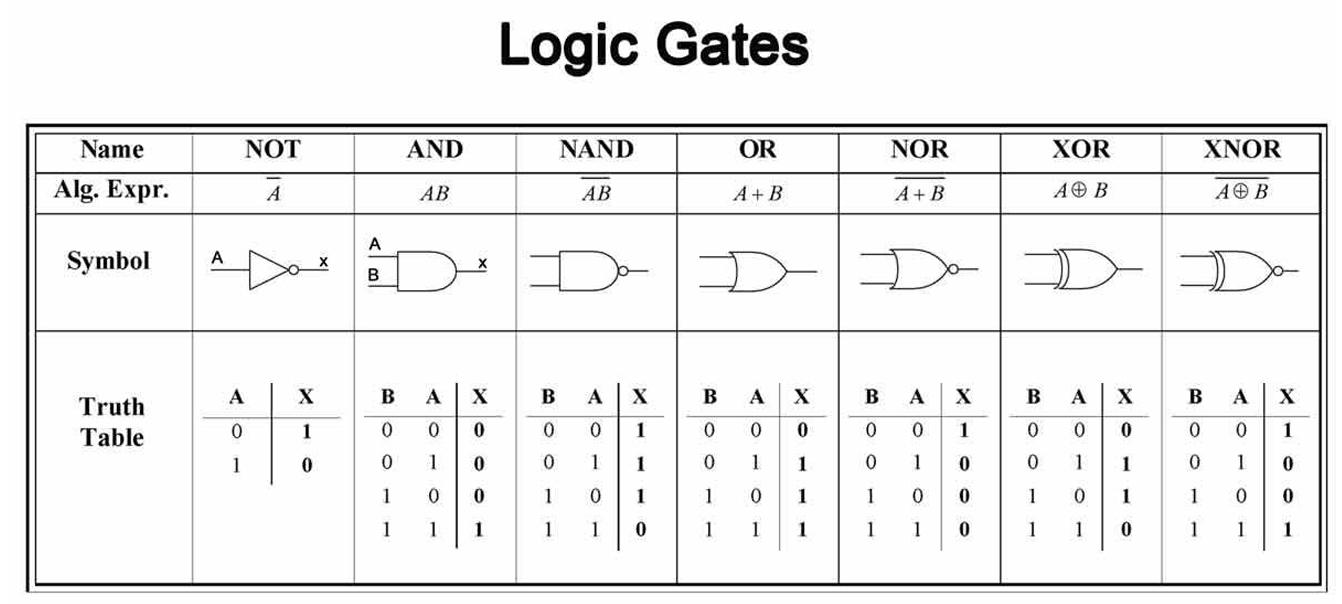
\includegraphics[width=0.8\textwidth]{images/logic_gates.png}
\caption{Logic Gates and Their Truth Tables}
\label{figure:logic-gates}
\end{figure}


\subsection{Operating System Fundamentals}
An operating system (OS) is a crucial software that manages a computer's resources and provides an interface between the hardware and user applications. At its core is the kernel, a critical component that handles low-level operations and directly interacts with the hardware.

\subsubsection{The Kernel}
\begin{itemize}
    \item \textbf{Definition:}
    \begin{itemize}
        \item The kernel is the central and most fundamental part of an operating system.
        \item It is responsible for managing hardware resources, including processors, memory, storage devices, and I/O.
    \end{itemize}
    \item \textbf{Resource Management:}
    \begin{itemize}
        \item Devices: Controls and communicates with hardware devices such as keyboards, mice, and printers.
    \end{itemize}
    \item \textbf{Interaction with Hardware:}
    \begin{itemize}
        \item The kernel provides an abstraction of the hardware, allowing applications to interact with hardware without needing to know the specific details of each device.
    \end{itemize}
\end{itemize}

\subsection{Operating System Functions}
\begin{itemize}
    \item \textbf{System Boot:}
    \begin{itemize}
        \item The boot process begins with the BIOS/UEFI, which loads the kernel into memory.
        \item The kernel starts execution and initiates the operating system's initialization process.
    \end{itemize}
    \item \textbf{Kernel Initialization:}
    \begin{itemize}
        \item During initialization, the kernel configures device drivers.
    \end{itemize}
    \item \textbf{Process Management:}
    \begin{itemize}
        \item When an application is started, the kernel creates a process for it.
        \item The kernel allocates resources and schedules the process to execute instructions on the CPU.
    \end{itemize}
    \item \textbf{Memory Management:}
    \begin{itemize}
        \item The kernel controls memory management.
    \end{itemize}
    \item \textbf{Device Communication:}
    \begin{itemize}
        \item The kernel handles I/O requests, interacting with device drivers to send and receive data to and from devices.
    \end{itemize}
\end{itemize}

\subsubsection{User Interface Interaction}
\begin{itemize}
    \item \textbf{User Interface:}
    \begin{itemize}
        \item The user interface, which can be a Command-Line Interface (CLI) or a Graphical User Interface (GUI), relies on the kernel to perform operations requested by users.
    \end{itemize}
    \item \textbf{Kernel Communication:}
    \begin{itemize}
        \item User applications communicate with the kernel through system calls, requesting specific services such as file reading/writing, memory allocation, etc.
    \end{itemize}
    \item \textbf{Application Management:}
    \begin{itemize}
        \item The kernel manages the execution of applications, ensuring that requested resources are accessed securely and controlled.
    \end{itemize}
\end{itemize}

\subsection{Scenario: System Boot and Application Launch on Windows}
\subsubsection{Phase 1: System Boot}
\begin{itemize}
    \item \textbf{Powering On the Computer:}
    \begin{itemize}
        \item The user powers on the computer with Windows OS installed.
        \item The boot process begins, managed by the bootloader and Windows kernel.
    \end{itemize}
    \item \textbf{Kernel Initialization:}
    \begin{itemize}
        \item The Windows kernel is loaded into memory and starts the initialization process.
        \item Configures device drivers, establishes system settings, and prepares the system for use.
    \end{itemize}
    \item \textbf{Loading the User Interface:}
    \begin{itemize}
        \item The kernel loads the Windows user interface, which may include the desktop and taskbar.
    \end{itemize}
\end{itemize}

\subsubsection{Phase 2: User Interface Interaction}
\begin{itemize}
    \item \textbf{Interacting with the User Interface:}
    \begin{itemize}
        \item The user interacts with the Windows UI, clicking on an application icon in the Start menu or on the desktop.
    \end{itemize}
    \item \textbf{Kernel Request:}
    \begin{itemize}
        \item The user interface sends a request to the Windows kernel to launch the selected application.
    \end{itemize}
    \item \textbf{Process Creation:}
    \begin{itemize}
        \item The Windows kernel creates a new process for the application, allocating resources such as memory and CPU time.
    \end{itemize}
\end{itemize}

\subsubsection{Phase 3: Application Management}
\begin{itemize}
\item \textbf{Application Execution:}
\begin{itemize}
\item The Windows kernel schedules the application’s process to execute on the CPU.
\item The application begins executing its instructions.
\end{itemize}
\item \textbf{Resource Management:}
\begin{itemize}
\item While the application is running, the kernel manages system resources, ensuring the application does not interfere with other processes or misuse resources.
\end{itemize}
\item \textbf{User Interface Communication:}
\begin{itemize}
\item The application communicates with the user interface through the Windows kernel to display output to the user and respond to interactions.
\end{itemize}
\end{itemize}


\subsection{Overview of Kernel Types in Operating Systems}
To reinforce our understanding of key concepts that will be covered in the upcoming slides, we will perform a quick review related to the kernel in general. These topics build a solid foundation for understanding advanced concepts and practical applications of the kernel within our training program.

\subsubsection{Types of Kernels}
There are several types of kernels, each with its unique architecture and functionality. Below are the main types of kernels:
\begin{itemize}
    \item \textbf{Microkernel}:
    A microkernel is a minimalistic kernel that includes only the most essential functionalities of an operating system. An example of a microkernel is \textit{MINIX}. In a microkernel architecture, many services such as device drivers, file systems, and network protocols are implemented in user space, which can lead to better modularity and reliability but may introduce performance overhead due to context switching between user space and kernel space.
    A microkernel, on the other hand, delegates many functionalities to processes in user space, keeping only the essential functions in the kernel itself. This design makes the system more modular and resilient to errors, as components can run in isolated user spaces. However, the communication between components across user-kernel boundaries can slow down performance.
    \item \textbf{Monolithic Kernel}:
    A monolithic kernel is a single binary file that includes most of the functionalities of an operating system. An example of a monolithic kernel is \textit{Unix}. Monolithic kernels run all operating system services in the kernel space, which allows for efficient system calls and better performance. However, this architecture can lead to stability issues, as a failure in one part of the kernel can crash the entire system.
    A monolithic kernel performs most operations directly in the kernel space, including memory management, process management, and communication between system components. This architecture is generally faster because system calls do not need to cross the boundary between user space and kernel space. However, it can lead to stability problems, as a bug in one part of the kernel can affect the entire system.
    \item \textbf{Modular Kernel}:
    A modular kernel can be seen as an extension of the monolithic kernel, with the capability to dynamically add or remove modules as needed. This provides a balance between performance and flexibility, allowing the kernel to be customized for different use cases without requiring a complete recompilation.
    \item \textbf{Hybrid Kernel: The Case of Windows}:
    The Windows kernel is a hybrid kernel, known as the \textit{Hybrid Kernel}. This means it incorporates elements of both monolithic and microkernel architectures.
    The hybrid approach in Windows combines elements of both architectures. For example, certain parts of the kernel, such as memory and process management, are implemented within the kernel itself (monolithic), while other functionalities, such as device drivers, can operate in user space (microkernel-like approach). This hybrid architecture aims to balance the speed of a monolithic kernel with the modularity and stability of a microkernel.
\end{itemize}


The kernel is the core of the operating system, efficiently managing hardware resources and providing a unified interface for user applications. Through precise orchestration of low-level operations, the kernel contributes to providing a stable and secure environment for running programs and interacting with hardware.


\subsection{Overview of Operating Systems}

An operating system (OS) is a software that provides services to users of a computer system and acts as an interface between the user and the physical machine. The primary tasks performed by an operating system include:

\begin{itemize}
    \item Memory management
    \item Process management, where a process is defined as a running program
    \item Process synchronization
    \item User interface management, such as handling input/output (I/O) operations for hardware peripherals like mice, keyboards, and screens
\end{itemize}


\subsubsection{Hardware and Operating System}
Hardware consists of the physical components that make up a personal computer, such as memory (RAM, hard drives, SSDs) and processors (CPUs) that are dedicated to executing instructions. The operating system is responsible for managing these components and providing a stable environment for applications to run.

To handle all these tasks, operating systems are generally composed of multiple modules, each dedicated to a specific function. The operating system organizes the interaction between these different modules, such as:

\begin{itemize}
    \item Process management
    \item I/O management
    \item File system management
    \item Central memory management
    \item User interface
\end{itemize}

\paragraph{Kernel}
The kernel is the core of the operating system, managing interactions between hardware and running processes. The file system is a mechanism that regulates the storage of data on a memory medium in an organized manner.

\section{Process Management}
A process is a running program, and each process is associated with a state, which can be:

\begin{itemize}
    \item \textbf{Running}: The process instructions are being executed by the processor (CPU).
    \item \textbf{Waiting}: The process is waiting for an event to occur (e.g., user input via keyboard).
    \item \textbf{Ready}: The process is waiting to be assigned to a processor to transition to the "Running" state.
    \item \textbf{Terminated}: The process has finished its execution.
\end{itemize}

The process manager module controls the synchronization and state of running programs. In a computer with multiple processes running simultaneously, each CPU executes the instructions of a process for a limited time before switching to another process. This switching of processes in the "Running" state is called scheduling, and the program that determines the time, manner, and sequence of switching is called the scheduler.

In modern multi-CPU systems, the process manager also handles the cooperation between different CPUs. Scheduling can be categorized into two types:

\begin{itemize}
    \item \textbf{Preemptive Scheduling}: The CPU currently in use by a process can be reassigned to execute another process at any time.
    \item \textbf{Cooperative Scheduling}: Once a process is in the "Running" state, it cannot be interrupted until it completes its work and voluntarily releases the CPU.
\end{itemize}

\subsection{Monotasking vs. Multitasking}
Monotasking operating systems can run only one program at a time. In such systems, the execution of a program cannot be suspended to assign the CPU to another program. These systems are generally outdated (e.g., MS-DOS). Monotasking systems are inefficient due to frequent periods of CPU idleness, as shown in the following graph:

\begin{figure}[h]
    \centering
    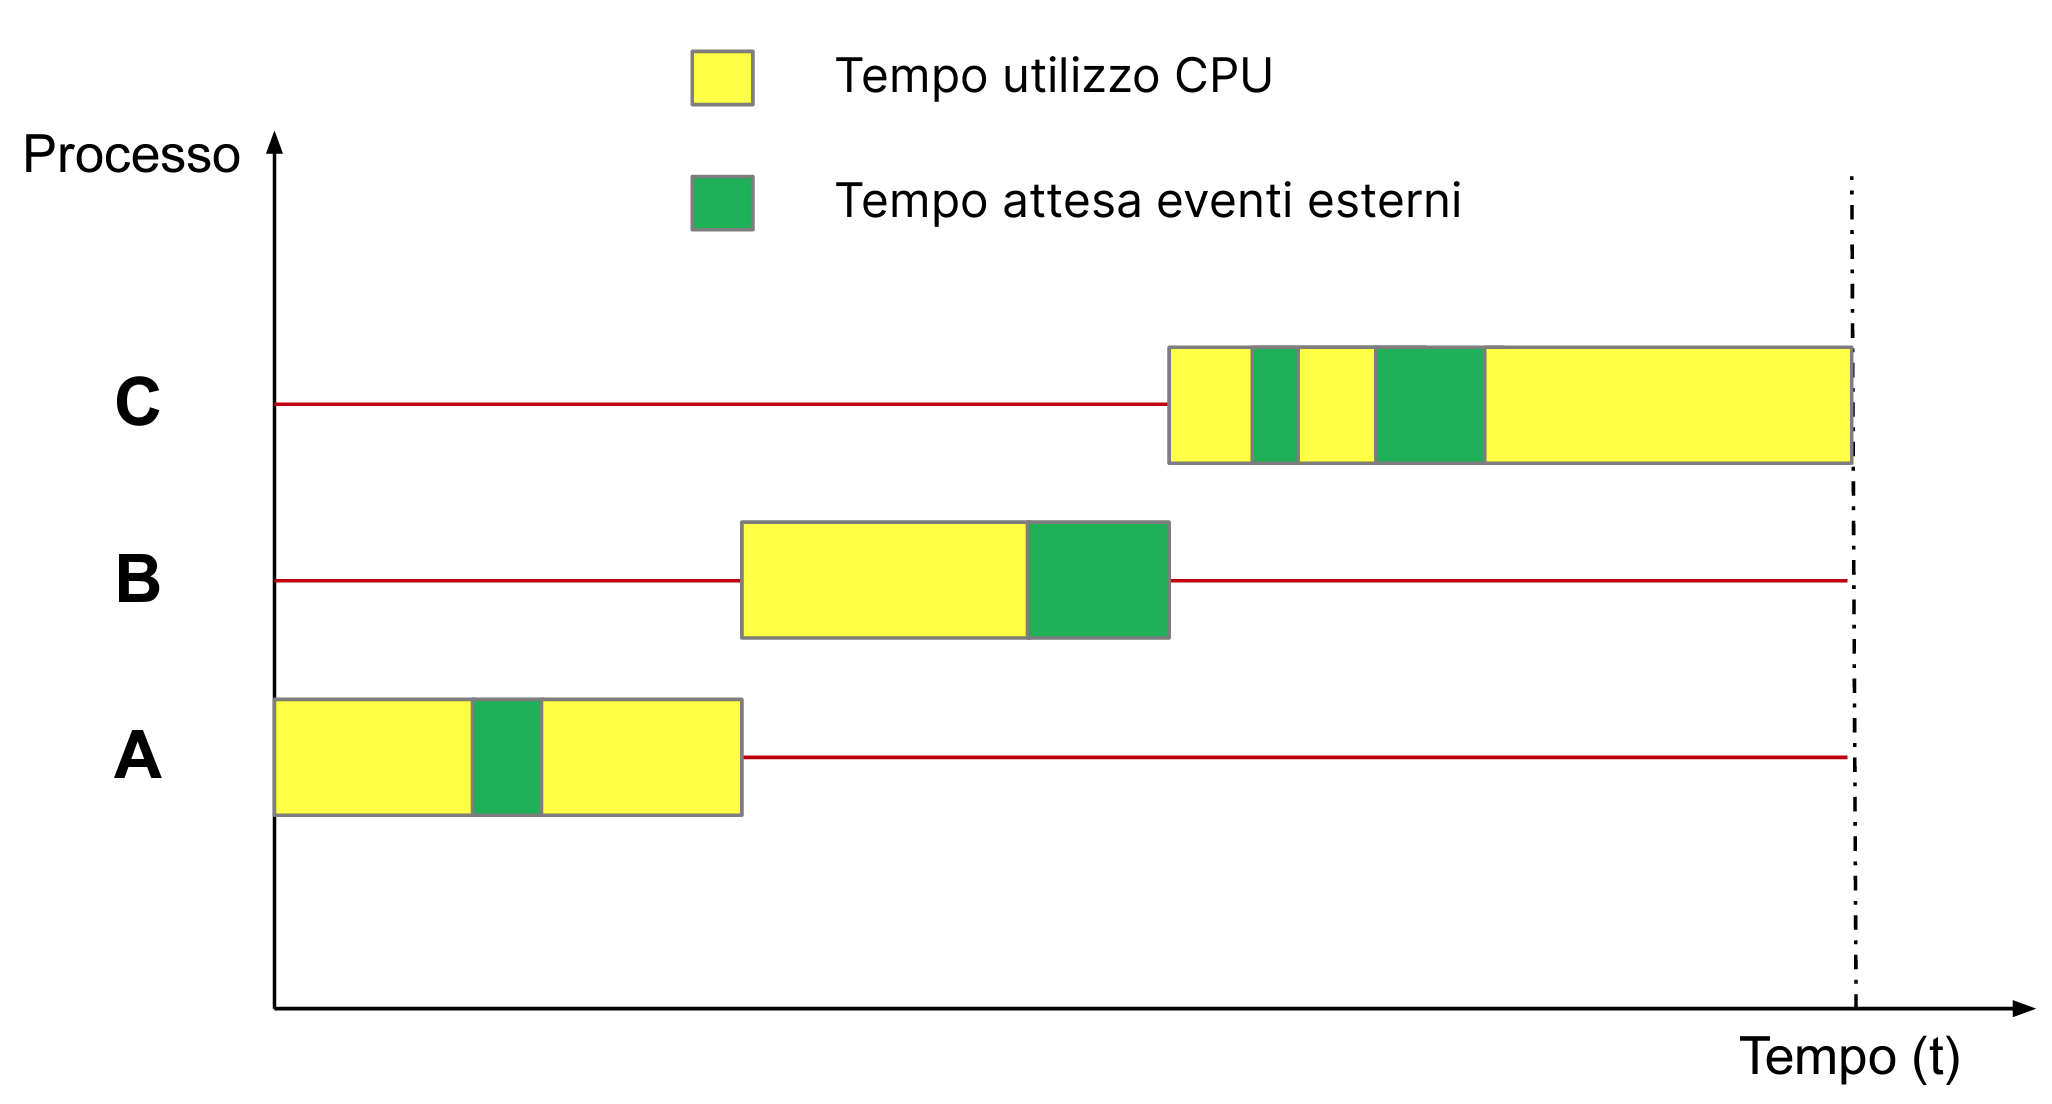
\includegraphics[width=0.8\textwidth]{images/monotask.png}
    \caption{Inefficiency of Monotasking Systems}
    \label{fig:monotasking_inefficiency}
\end{figure}

Multitasking operating systems allow the concurrent execution of multiple programs. Examples of multitasking operating systems include Windows-NT and Linux-based systems. In multitasking systems, processes can be interrupted to shift the CPU's attention to another process.

\begin{figure}[h]
    \centering
    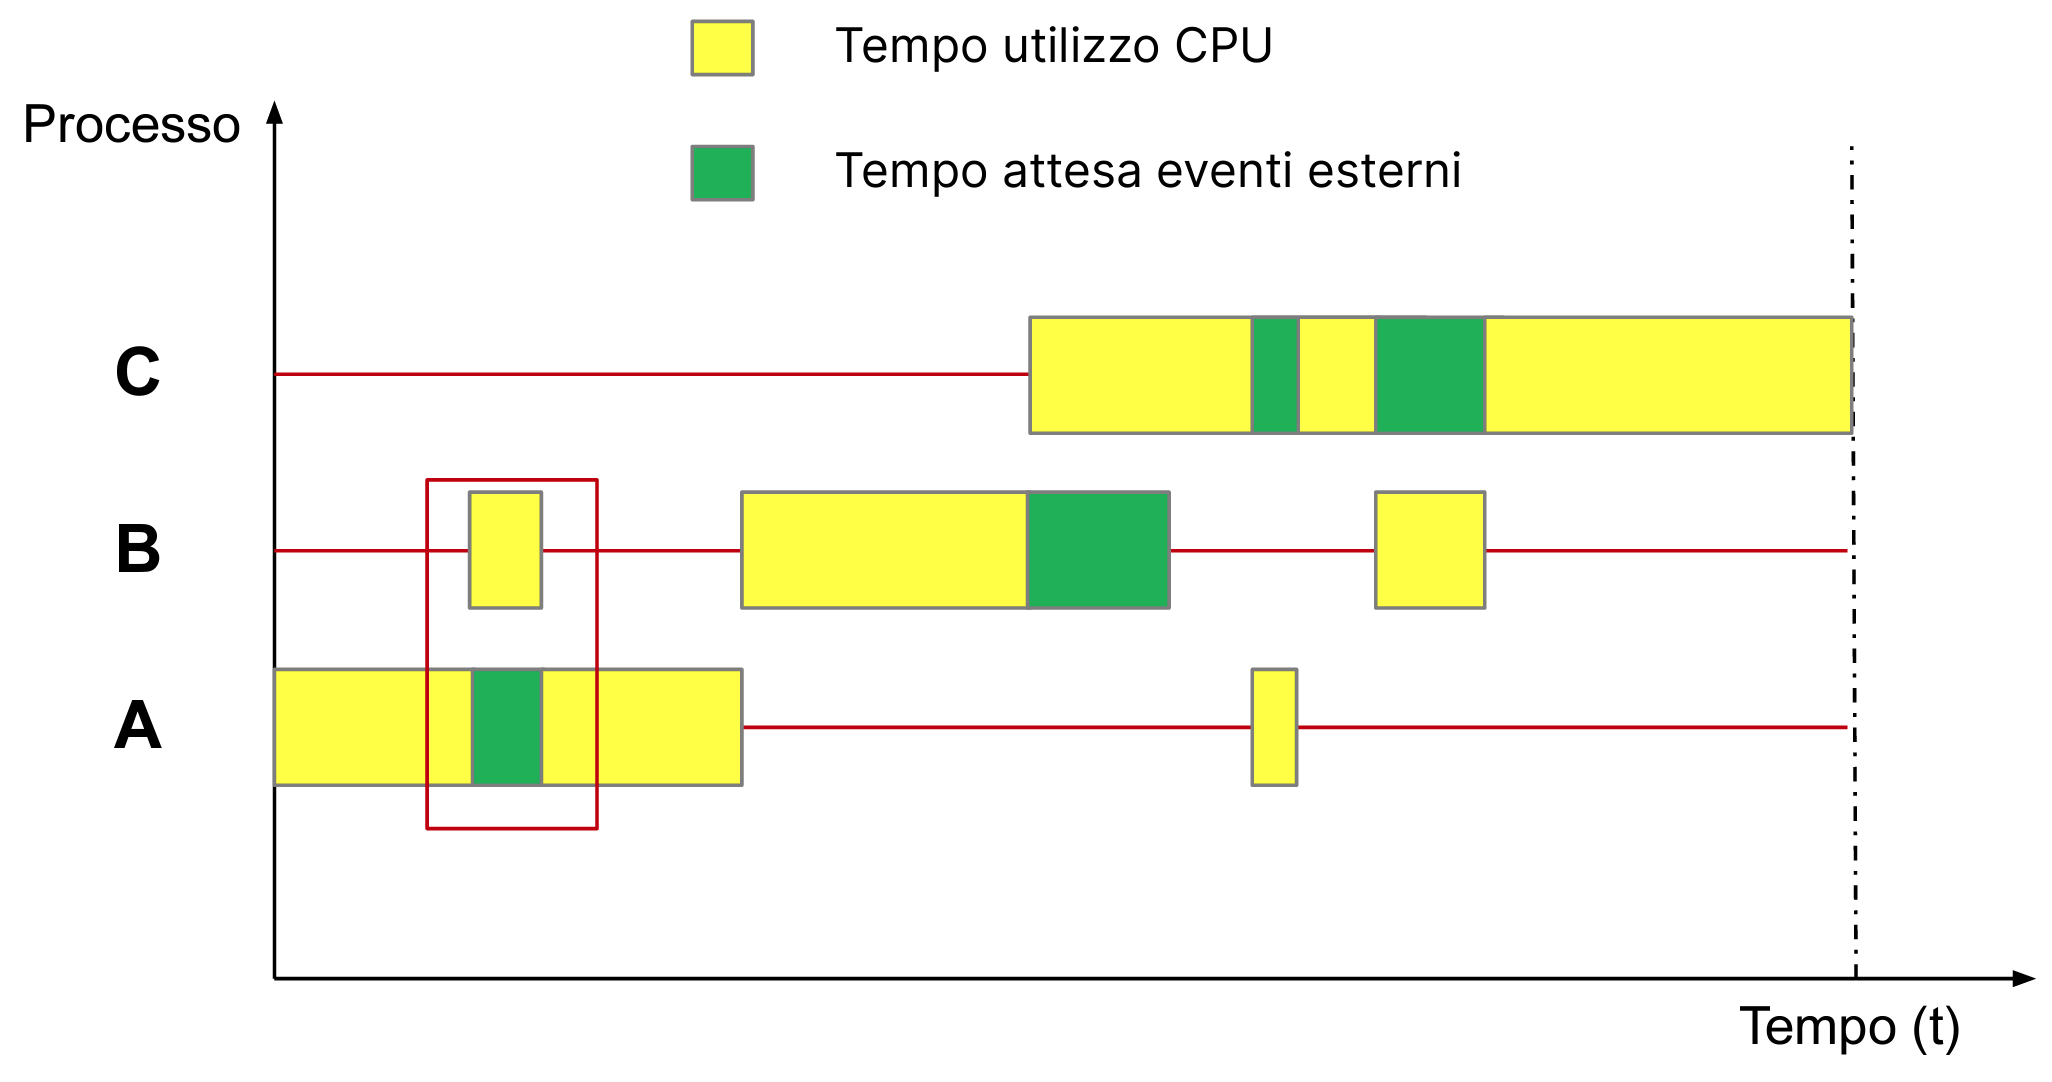
\includegraphics[width=0.8\textwidth]{images/multitask.png}
    \caption{Efficiency of Multitasking Systems}
    \label{fig:multitasking_efficiency}
\end{figure}

\subsection{Time-Sharing Systems}
An evolution of multitasking systems is time-sharing systems. In a time-sharing system, each process is executed cyclically for small time intervals called "time slices" or "quanta". With a sufficiently fast CPU, a time-sharing system gives the impression of parallel process evolution.

\begin{figure}[h]
    \centering
    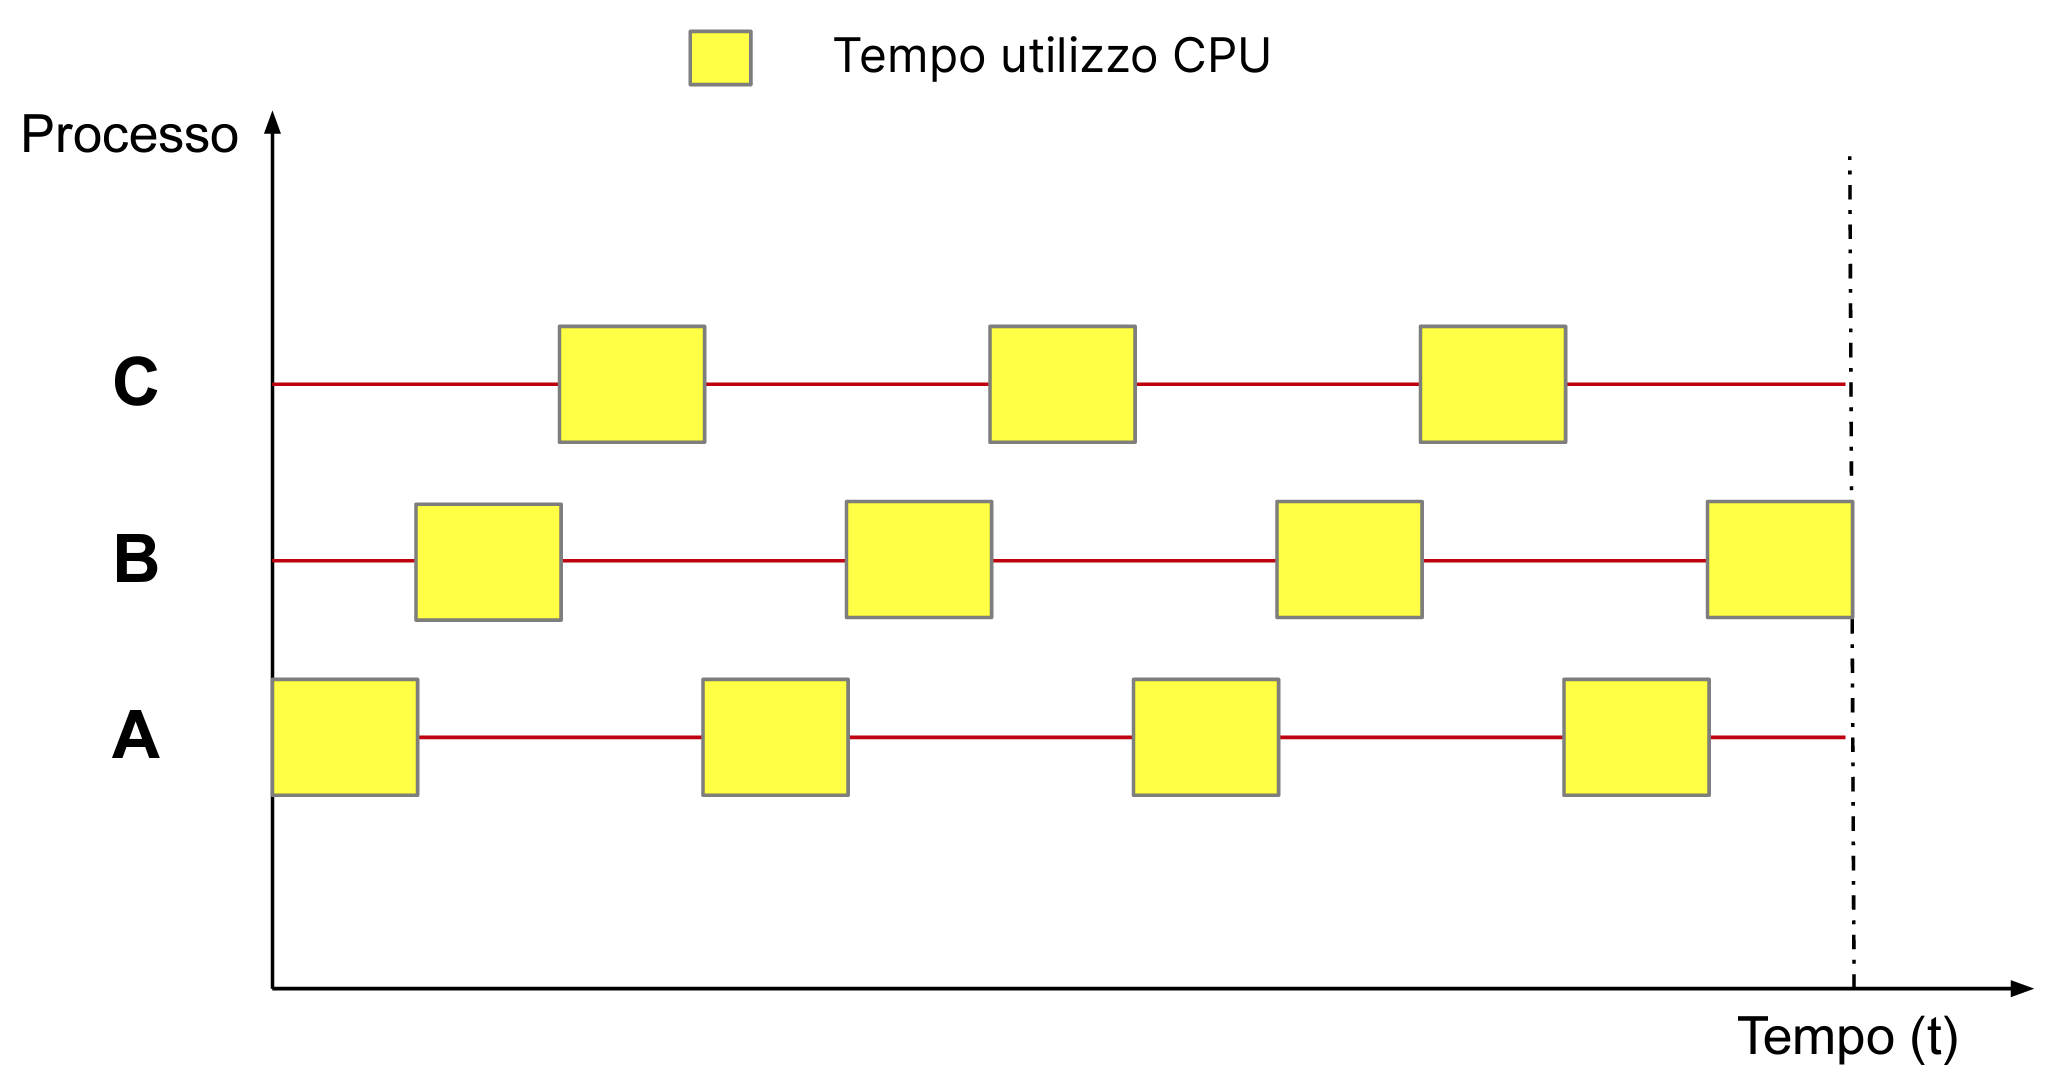
\includegraphics[width=0.8\textwidth]{images/timeshare.png}
    \caption{Time-Sharing System}
    \label{fig:time_sharing}
\end{figure}

In time-sharing systems, processes are executed for a standard period called a "quantum". The process is interrupted to execute another process for a "quantum", and so on.

\subsection{Preemptive and Cooperative Multitasking}
Common operating systems, such as Windows, macOS, and many Linux distributions, adopt preemptive multitasking to manage the simultaneous execution of multiple processes or applications. There are two main types of multitasking:

\begin{itemize}
    \item \textbf{Preemptive Multitasking}: In a preemptive multitasking system, the operating system allocates a certain period (time slice or quantum) to each process and then automatically switches to the next process. This approach is called "preemptive" because the operating system can interrupt a running process before it completes its execution period. This ensures fair distribution of system resources among processes.
    \item \textbf{Cooperative Multitasking}: In a cooperative multitasking system, it is the responsibility of individual processes to release control of the CPU when they no longer need it. This requires greater cooperation among processes, as they must be designed to voluntarily yield control. However, if a process does not release control, it can negatively impact system performance.
\end{itemize}

The operating system is a crucial software component that provides services to users and acts as an interface between the user and the physical machine. By managing hardware resources efficiently and providing a stable environment for applications, the operating system plays a vital role in the overall functionality and performance of a computer system.


\subsection{Memory Management in Operating Systems}
One of the central and most important tasks of an operating system is the management of central memory. But what is central memory? We can distinguish four types of central memory:

\begin{itemize}
    \item ROM (Read Only Memory): ROM is used by operating systems for computer initialization programs. Basic routines of computer systems, such as the BIOS (Basic Input/Output System), were traditionally written in ROM. Today, it is more accurate to refer to this type of memory as EEPROM.
    \item CPU Registers: CPU registers are very fast access memory locations used by the CPU to store instructions to be followed for short periods of time.
    \item Cache Memory: Cache memory represents areas where previously used data is temporarily stored for faster future access. Cache memories are quite limited and can only contain a small amount of data.
    \item RAM (Random Access Memory): RAM is the main memory of an operating system, and the greater the available amount, the better the PC's performance. RAM consists of a matrix of cells, each identified by an address in binary notation. When a process is executed by the CPU, its instructions, saved on secondary memory, must be loaded into RAM cells to be read.
\end{itemize}

Secondary memory, or mass memory, refers to non-volatile memory types (i.e., where information remains saved even when the machine is turned off). Examples include hard disks, USB flash drives, and SSDs.


\subsection{Memory Management Module}
The memory manager is the module responsible for allocating memory to various tasks when needed and removing tasks from memory when completed. The complexity of the memory manager is directly related to the type of operating system. In multi-tasking systems, managing multiple programs loaded in memory is more complex, particularly the optimal allocation of memory spaces.

\subsubsection{Linear Allocation Example}
Consider a multi-tasking system with three processes, A, B, and C.

\begin{enumerate}
    \item Process A transitions to the running state, and the CPU loads A's instructions into RAM.
    \item Next, it is B's turn, and the CPU loads B's instructions.
    \item The instructions of C are then loaded into memory.
\end{enumerate}

This model is known as linear allocation. The memory blocks occupied by each process depend on the number of instructions each process needs to execute.

\paragraph{Fragmentation Issue}
Consider the following scenario:
\begin{enumerate}
    \item Process C completes its work, and the CPU removes it from memory.
    \item Process D needs to be executed, but the memory space it requires is larger than what was freed by C. As a result, there will be unused free memory until a process that fits into the space freed by C can be found.
\end{enumerate}

\paragraph{Paging Solution}
The solution to the fragmentation problem is "paging." With this technique, memory is divided into blocks of equal size, called "pages." Each process that needs to be executed is allocated a portion of memory equal to one or more pages.

In this way, memory is used optimally, without free spaces.

\subsection{Virtual Memory}
There are situations where the memory is insufficient to hold all the processes. The concept of virtual memory is introduced, where the operating system creates what appears to be dedicated memory for each process. Only the necessary parts of code and data for the process are loaded into memory, while the rest is moved to a secondary memory area called the "swap area."

\begin{figure}[h]
    \centering
    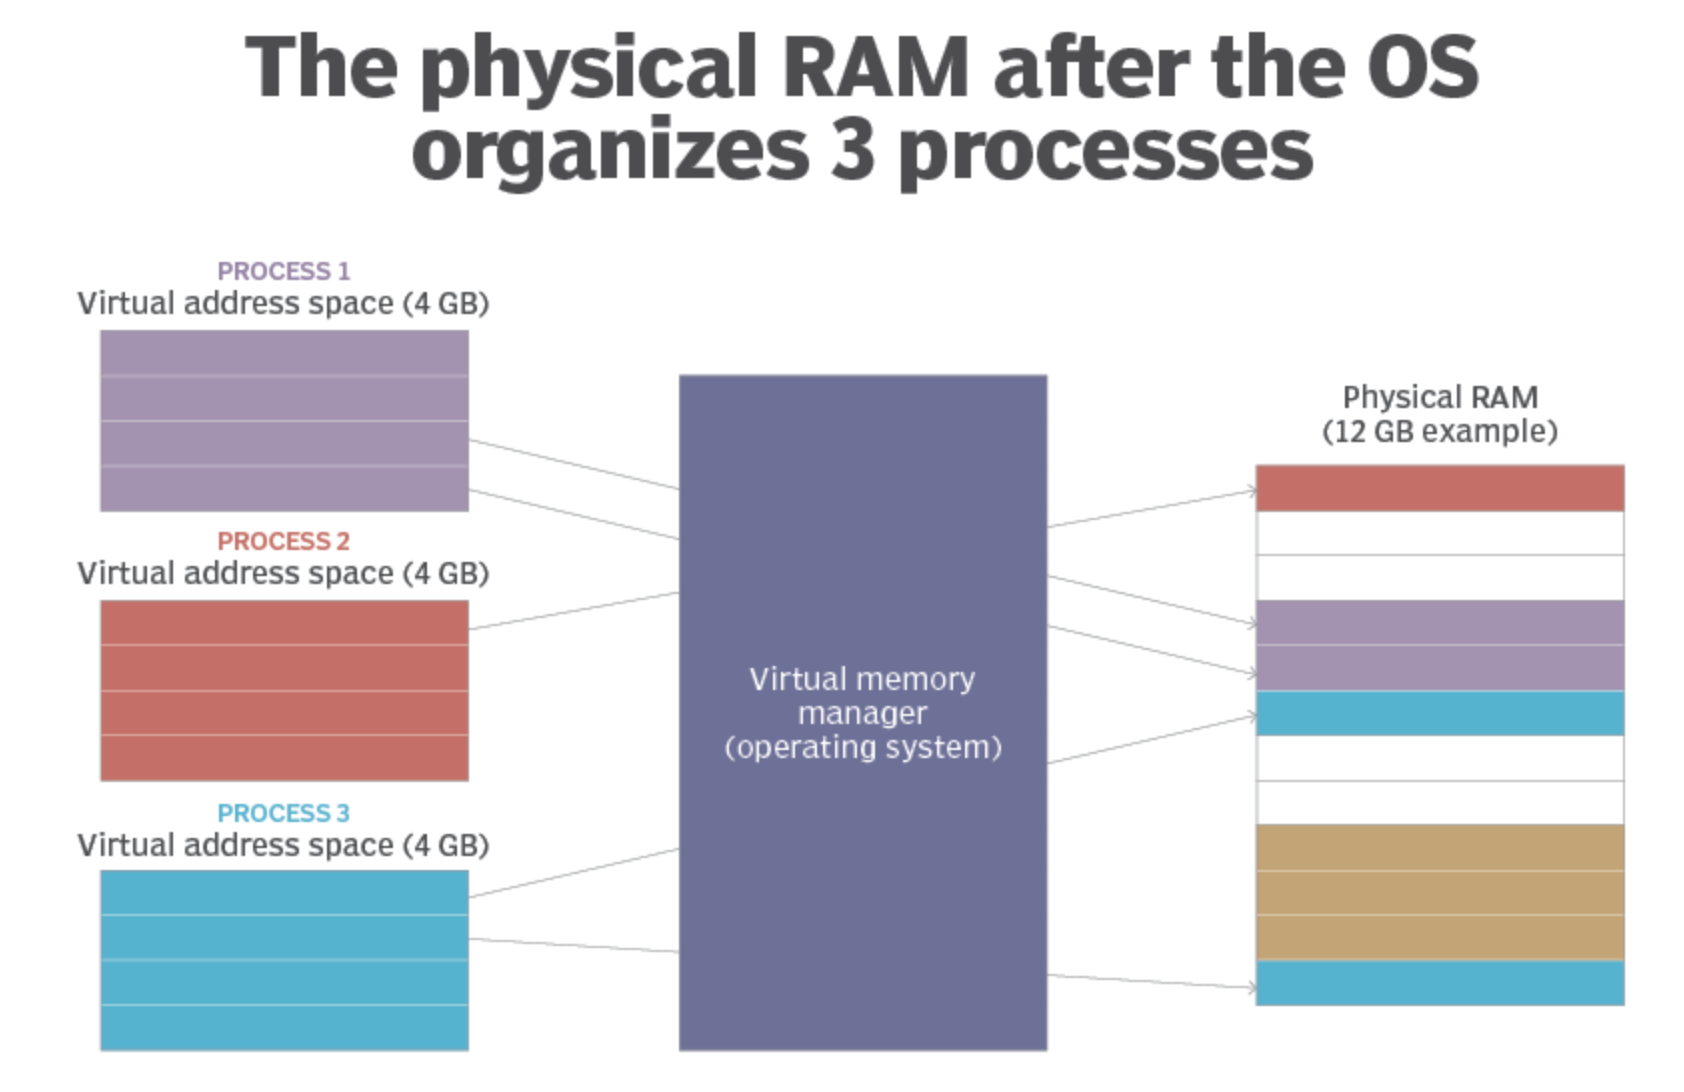
\includegraphics[width=0.8\textwidth]{images/memory.png}
    \caption{Virtual Memory Management}
    \label{fig:virtual_memory}
\end{figure}

The mehanisms for implementing virtual memory are complex, but modern processors have hardware mechanisms to facilitate its management.


Memory management is a critical function of an operating system, involving the efficient allocation and deallocation of memory resources to various processes. Techniques like paging and virtual memory help optimize memory usage and improve overall system performance, ensuring that the system can handle multiple tasks efficiently and effectively.

\subsection{File Systems in Operating Systems}
The file system manager is a module of the operating system responsible for managing information stored on secondary storage devices, also known as mass storage. Secondary storage refers to non-volatile memory, where stored data is permanent and does not depend on the state of the computer (on or off). The main role of the file system manager is to control and ensure the correctness and consistency of the information. Various technologies today offer different file systems to users, such as FAT32, NTFS, Apple File System, ext3, and ext4. Regardless of the technology, almost all file systems use a hierarchical approach, where directories are used to group multiple files together.

\subsubsection{Key Concepts of File Systems}
Here are some key concepts related to file systems:

\begin{itemize}
    \item File: a file is a logical unit of data containing information such as text, images, programs, or data.

    \item Directory (Folder): a directory is a logical container for files and other directories. Directories are organized in a tree structure, forming the hierarchy of a file system.

    \item Path: a path represents the location of a file or directory within the file system. For example, \texttt{C:\textbackslash Users\textbackslash username\textbackslash Documents} is a path in a Windows file system.

    \item Hierarchy: the directory structure forms a hierarchy that simplifies the organization of files in an orderly manner.
\end{itemize}

\paragraph{Types of File Systems}
There are various types of file systems, each with its own characteristics and uses. Some examples include NTFS (New Technology File System) and FAT32 on Windows systems, HFS+ on macOS, and ext4 on Linux systems.

\paragraph{Formatting}
Formatting a storage device creates a file system on it, preparing it for use. Formatting can affect the type of file system used.

\paragraph{Access and Security}
File systems often handle access control and data security, defining who can read, write, or execute certain files or directories.

In summary, the file system is a crucial component of any operating system, providing an organizational structure for efficiently storing and retrieving data.

\subsection{I/O Device Manager}
The Input/Output (I/O) device manager is a module of the operating system responsible for allocating devices to processes that request access, such as the mouse, keyboard, screen, and so on. To do this, the I/O device manager relies on software called "drivers" (you may have heard the term: "you need to download/update drivers for video cards, for example"), which are generally released by device manufacturers.

\subsubsection{Driver Functions}
Some main tasks performed by a driver include:

\begin{itemize}
    \item Managing signals to external peripherals (screens, keyboards, mice, etc.).
    \item Handling conflicts and synchronization when two processes need the same device simultaneously.
\end{itemize}

When a process requests access to an I/O device, the driver checks its status. If it is available, it assigns it to the process and marks the device as "busy." This way, synchronization problems between processes that request the same device simultaneously are avoided.

\subsection{User Experience}
One of the primary goals of operating systems is to support users and facilitate their tasks. All operating systems implement mechanisms to make the "user experience" easier, i.e., the use of the system by users. The user interface is what simplifies the interaction between users and hardware systems. Two categories of user interfaces can be distinguished:

\subsubsection{Textual User Interface}
Examples include command interpreters on Linux (shell) or PowerShell on Windows.

\subsubsection{Graphical User Interface}
The program outputs are displayed on the screen within windows.

The file system manager, I/O device manager, and user interface are crucial components of any operating system. They work together to provide an efficient, secure, and user-friendly environment for managing hardware resources and data. By understanding these components, we can appreciate the complex orchestration that allows modern operating systems to function seamlessly.

\subsection{Security in Operating Systems}

When discussing operating system security, it is essential to consider the external environment in which the system operates to determine appropriate security measures. A server running a critical application in a server room will certainly need physical security policies, such as being housed in a locked room with surveillance mechanisms. In contrast, a personal computer does not require a server room but must be protected from threats such as:

\begin{itemize}
    \item Unauthorized access
    \item Data modification or deletion
    \item Theft of confidential information
\end{itemize}


\subsubsection{Authentication}
Authentication is a process aimed at recognizing the user on a computer system. Generally, authentication is verified through login mechanisms that use credentials, which can be public like the username and secret like the password. To enhance the security of the login process, passwords are often subject to password security policies, which include a series of requirements, such as:

\begin{itemize}
    \item Password length: at least 8 characters
    \item Password complexity: at least one uppercase letter, one number, one symbol
    \item Password rarity: avoiding common passwords like \texttt{Password1!} or repeated characters
    \item Periodic password change: for example, every 3 months
\end{itemize}

In the authentication process, two main actors are involved:

\begin{itemize}
    \item The user who enters the credentials
    \item The authentication system, which verifies the credentials provided by the user
\end{itemize}

An authentication system verifies the user by comparing the credentials entered by the user with the credentials stored in a dedicated directory used to store data for all users who have access to the system, known as the \textit{user repository}.

There are two critical security aspects to consider in this process:

\begin{itemize}
    \item Credentials in the user repository must be stored encrypted, not in plaintext.
    \item Credentials in transit at points 2 and 3 should be either encrypted or transmitted over a secure channel.
\end{itemize}

Ensuring that data is encrypted both in transit between systems and when stored statically on a system is fundamental.

\subsubsection{Basic Authentication}
The example above illustrates basic authentication, as it uses only one step of authentication. For more sensitive applications, additional authentication methods can be added to provide an extra layer of security. Nowadays, the use of passwords alone is highly discouraged, and Multi-Factor Authentication (MFA) is strongly recommended. A second authentication factor, in addition to the password, could be one of the following:

\begin{itemize}
    \item \textbf{Something the user has}: e.g., a phone for authentication via push notification, app, or QR code.
    \item \textbf{Something the user knows}: e.g., a second factor such as a PIN.
    \item \textbf{Something the user is}: e.g., a second factor such as a physical characteristic, like facial recognition or fingerprint.
\end{itemize}

\subsubsection{Examples of Second Authentication Factors}
The use of a second authentication factor significantly enhances security because an attacker would need both your password and your second authentication method. Examples include Google and Microsoft Authenticator apps, which provide one-time codes, and banking apps that require a second authentication step for transactions.

\begin{table}[h]
    \centering
    \begin{tabular}{|l|l|}
    \hline
    \textbf{Second Factor} & \textbf{Description} \\ \hline
    Push notification – mobile app & The user receives a one-time code on a smartphone app \\ \hline
    USB Token & A hardware device generating a unique code \\ \hline
    Fingerprint/Facial recognition & Physical characteristic used as a second factor \\ \hline
    Phone call & The user receives a call with a numerical code \\ \hline
    \end{tabular}
    \caption{Examples of Second Authentication Factors}
    \label{tab:second_authentication_factors}
\end{table}


\subsubsection{Authorization}
While authentication handles user verification, authorization manages the privileges of a verified user. Authorization defines access rights to resources, such as read/write permissions on a file or executing a specific task. It is important to note that authorization follows authentication; once the user is verified, they are granted or denied permission to perform certain functions based on their privileges.

\paragraph{Access Control Models}
Authorization can be defined at the operating system level using one of the following models:

\begin{itemize}
    \item \textbf{Discretionary Access Control (DAC)}: Uses a decentralized model where the owner of a document can manage its privileges.
    \item \textbf{Mandatory Access Control (MAC)}: Uses a centralized model, assigning security labels to resources to classify information and specify authorized user groups.
    \item \textbf{Role-Based Access Control (RBAC)}: Assigns privileges based on user roles, adhering to the principle of least privilege.
\end{itemize}

\subsubsection{Accounting}
Accounting allows tracking of resource usage by a user. An example of accounting is system logs, which track events such as logins, logouts, and configuration changes for each user accessing the system. Given that most attacks on companies originate from internal users, accounting is crucial for identifying the perpetrators of malicious activities. For example, if your account is compromised through phishing, logs can trace all malicious activities performed with your account and possibly even the attempt to steal your credentials, thus protecting you from being held responsible.

Security in operating systems encompasses various aspects, including physical security, authentication, authorization, and accounting. By understanding and implementing these security measures, we can ensure a robust defense against both external and internal threats, providing a secure and reliable environment for users and applications.








% And this is a nice \texttt{\$\$...\$\$} display environment:
% $$
% \Delta v = \int\displaylimits_{t_0}^{t_1} a \, \textrm{d}t
% $$
% Maecenas ut nisi condimentum nisi iaculis porttitor eu sed metus. Proin faucibus aliquet odio, ac lobortis tortor. Mauris porta molestie tortor blandit pretium. Nulla pulvinar id mauris ut efficitur. Donec posuere tortor a odio pellentesque tincidunt. Nulla mi nunc, accumsan nec lectus ut, euismod vulputate libero.
% %
% And finally we have the \texttt{align/align*} environment:
% \begin{align}
% x_f - x_i &= \bar{v}t \nonumber\\
% \Rightarrow s &= \bar{v}t
% \end{align}
% %
% \section{Yet another section}
% \subsection{And a subsection beneath it}
% \lecture[1 hour]{13}{06}{2017}
% %
% \subsection{And now a subsection}
% \subsubsection{With a subsubsection following it}
% %
% Integer pharetra nulla scelerisque purus luctus iaculis. Mauris pulvinar erat non dui pretium, sed vestibulum sapien condimentum. Nam in urna quis sapien rhoncus placerat vitae sit amet odio. Vivamus finibus euismod nibh vestibulum lobortis.\margintext{These ideas were probably discussed in lecture 1 in a parallel universe.} Integer arcu tortor, vestibulum sit amet iaculis ut, ullamcorper non ante. Pellentesque consectetur nec odio quis placerat. Vestibulum vehicula massa vel euismod blandit.
% %
% %
% \margintext{\protect\vspace{2cm}Table \ref{tab:mori} courtesy of Mori, L.F. `Tables in \LaTeX2$\epsilon$: Packages and Methods'.}
% \begin{table}[h]
% \centering
% \begin{tabular}{clcc}
% \toprule
% \multicolumn{2}{c}{$D$} & $P_u$ & $\sigma_N$\\
% \multicolumn{2}{c}{(in)} & (lbs) & (psi)\\\toprule
% \multirow{3}*{5} & test 1 & 285 & 38.00\\\cmidrule(l){2-4}
% & test 2 & 287 & 38.27\\\cmidrule(l){2-4}
% & test 3 & 230 & 30.67\\\midrule
% \multirow{3}*{10} & test 1 & 430 & 28.67\\\cmidrule(l){2-4}
% & test 2 & 433 & 28.87\\\cmidrule(l){2-4}
% & test 3 & 431 & 28.73\\\bottomrule
% \end{tabular}
% \caption{A table beautified by the \protect\texttt{booktabs} package.}\label{tab:mori}
% \end{table}
% %
% %
% \subsubsection{This subsubsection is all by itself}
% %
% \vskip7ex
% \centering
* * *
%
\end{document}%
